\documentclass[a4paper]{book}
\usepackage{a4wide}
\usepackage{makeidx}
\usepackage{graphicx}
\usepackage{multicol}
\usepackage{float}
\usepackage{listings}
\usepackage{color}
\usepackage{textcomp}
\usepackage{alltt}
\usepackage{times}
\usepackage{ifpdf}
\ifpdf
\usepackage[pdftex,
            pagebackref=true,
            colorlinks=true,
            linkcolor=blue,
            unicode
           ]{hyperref}
\else
\usepackage[ps2pdf,
            pagebackref=true,
            colorlinks=true,
            linkcolor=blue,
            unicode
           ]{hyperref}
\usepackage{pspicture}
\fi
\usepackage[utf8]{inputenc}
\usepackage{doxygen}
\lstset{language=C++,inputencoding=utf8,basicstyle=\footnotesize,breaklines=true,breakatwhitespace=true,tabsize=8,numbers=left }
\makeindex
\setcounter{tocdepth}{3}
\renewcommand{\footrulewidth}{0.4pt}
\begin{document}
\hypersetup{pageanchor=false}
\begin{titlepage}
\vspace*{7cm}
\begin{center}
{\Large mmplot \\[1ex]\large 0.1b }\\
\vspace*{1cm}
{\large Generated by Doxygen 1.6.2}\\
\vspace*{0.5cm}
{\small Sat Mar 27 08:35:31 2010}\\
\end{center}
\end{titlepage}
\clearemptydoublepage
\pagenumbering{roman}
\tableofcontents
\clearemptydoublepage
\pagenumbering{arabic}
\hypersetup{pageanchor=true}
\chapter{Namespace Index}
\section{Namespace List}
Here is a list of all namespaces with brief descriptions:\begin{DoxyCompactList}
\item\contentsline{section}{\hyperlink{namespaceGtk}{Gtk} }{\pageref{namespaceGtk}}{}
\item\contentsline{section}{\hyperlink{namespaceGtk_1_1Plot}{Gtk::Plot} }{\pageref{namespaceGtk_1_1Plot}}{}
\end{DoxyCompactList}

\chapter{Class Index}
\section{Class Hierarchy}
This inheritance list is sorted roughly, but not completely, alphabetically:\begin{DoxyCompactList}
\item \contentsline{section}{Gtk::Plot::Area}{\pageref{classGtk_1_1Plot_1_1Area}}{}
\item \contentsline{section}{Gtk::Plot::Border}{\pageref{structGtk_1_1Plot_1_1Border}}{}
\item \contentsline{section}{Gtk::Plot::Container}{\pageref{classGtk_1_1Plot_1_1Container}}{}
\item \contentsline{section}{Gtk::Plot::Drawable}{\pageref{classGtk_1_1Plot_1_1Drawable}}{}
\begin{DoxyCompactList}
\item \contentsline{section}{Gtk::Plot::DrawableData$<$ DataPoint2D $>$}{\pageref{classGtk_1_1Plot_1_1DrawableData}}{}
\begin{DoxyCompactList}
\item \contentsline{section}{Gtk::Plot::Line2D}{\pageref{classGtk_1_1Plot_1_1Line2D}}{}
\end{DoxyCompactList}
\item \contentsline{section}{Gtk::Plot::DrawableData$<$ T $>$}{\pageref{classGtk_1_1Plot_1_1DrawableData}}{}
\item \contentsline{section}{Gtk::Plot::PlotLineDataStruct2D}{\pageref{structGtk_1_1Plot_1_1PlotLineDataStruct2D}}{}
\end{DoxyCompactList}
\end{DoxyCompactList}

\chapter{Class Index}
\section{Class List}
Here are the classes, structs, unions and interfaces with brief descriptions:\begin{DoxyCompactList}
\item\contentsline{section}{\hyperlink{classGtk_1_1Plot_1_1Area}{Gtk::Plot::Area} }{\pageref{classGtk_1_1Plot_1_1Area}}{}
\item\contentsline{section}{\hyperlink{structGtk_1_1Plot_1_1Border}{Gtk::Plot::Border} }{\pageref{structGtk_1_1Plot_1_1Border}}{}
\item\contentsline{section}{\hyperlink{classGtk_1_1Plot_1_1Container}{Gtk::Plot::Container} }{\pageref{classGtk_1_1Plot_1_1Container}}{}
\item\contentsline{section}{\hyperlink{classGtk_1_1Plot_1_1Drawable}{Gtk::Plot::Drawable} }{\pageref{classGtk_1_1Plot_1_1Drawable}}{}
\item\contentsline{section}{\hyperlink{classGtk_1_1Plot_1_1DrawableData}{Gtk::Plot::DrawableData$<$ T $>$} }{\pageref{classGtk_1_1Plot_1_1DrawableData}}{}
\item\contentsline{section}{\hyperlink{classGtk_1_1Plot_1_1Line2D}{Gtk::Plot::Line2D} }{\pageref{classGtk_1_1Plot_1_1Line2D}}{}
\item\contentsline{section}{\hyperlink{structGtk_1_1Plot_1_1PlotLineDataStruct2D}{Gtk::Plot::PlotLineDataStruct2D} }{\pageref{structGtk_1_1Plot_1_1PlotLineDataStruct2D}}{}
\end{DoxyCompactList}

\chapter{File Index}
\section{File List}
Here is a list of all files with brief descriptions:\begin{DoxyCompactList}
\item\contentsline{section}{\hyperlink{DrawableData_8cpp}{DrawableData.cpp} }{\pageref{DrawableData_8cpp}}{}
\item\contentsline{section}{\hyperlink{DrawableData_8h}{DrawableData.h} }{\pageref{DrawableData_8h}}{}
\item\contentsline{section}{\hyperlink{Line2D_8cpp}{Line2D.cpp} }{\pageref{Line2D_8cpp}}{}
\item\contentsline{section}{\hyperlink{Line2D_8h}{Line2D.h} }{\pageref{Line2D_8h}}{}
\item\contentsline{section}{\hyperlink{PlotArea_8cpp}{PlotArea.cpp} }{\pageref{PlotArea_8cpp}}{}
\item\contentsline{section}{\hyperlink{PlotArea_8h}{PlotArea.h} }{\pageref{PlotArea_8h}}{}
\item\contentsline{section}{\hyperlink{PlotContainer_8cpp}{PlotContainer.cpp} }{\pageref{PlotContainer_8cpp}}{}
\item\contentsline{section}{\hyperlink{PlotContainer_8h}{PlotContainer.h} }{\pageref{PlotContainer_8h}}{}
\item\contentsline{section}{\hyperlink{types_8h}{types.h} }{\pageref{types_8h}}{}
\end{DoxyCompactList}

\chapter{Namespace Documentation}
\hypertarget{namespaceGtk}{
\section{Gtk Namespace Reference}
\label{namespaceGtk}\index{Gtk@{Gtk}}
}
\subsection*{Namespaces}
\begin{DoxyCompactItemize}
\item 
namespace \hyperlink{namespaceGtk_1_1Plot}{Plot}
\end{DoxyCompactItemize}

\hypertarget{namespaceGtk_1_1Plot}{
\section{Gtk::Plot Namespace Reference}
\label{namespaceGtk_1_1Plot}\index{Gtk::Plot@{Gtk::Plot}}
}
\subsection*{Classes}
\begin{DoxyCompactItemize}
\item 
class \hyperlink{classGtk_1_1Plot_1_1Area}{Area}
\item 
struct \hyperlink{structGtk_1_1Plot_1_1Border}{Border}
\item 
class \hyperlink{classGtk_1_1Plot_1_1Container}{Container}
\item 
class \hyperlink{classGtk_1_1Plot_1_1Drawable}{Drawable}
\item 
class \hyperlink{classGtk_1_1Plot_1_1DrawableData}{DrawableData}
\item 
class \hyperlink{classGtk_1_1Plot_1_1Line2D}{Line2D}
\item 
struct \hyperlink{structGtk_1_1Plot_1_1PlotLineDataStruct2D}{PlotLineDataStruct2D}
\end{DoxyCompactItemize}
\subsection*{Typedefs}
\begin{DoxyCompactItemize}
\item 
typedef \hyperlink{structGtk_1_1Plot_1_1PlotLineDataStruct2D}{Gtk::Plot::PlotLineDataStruct2D} \hyperlink{namespaceGtk_1_1Plot_abea92d3a790b1bcf6a64f98511231815}{DataPoint2D}
\item 
typedef \hyperlink{structGtk_1_1Plot_1_1Border}{Border} \hyperlink{namespaceGtk_1_1Plot_a9b9ee0ab9bbec47945b0bf70f30ea308}{Line}
\end{DoxyCompactItemize}
\subsection*{Enumerations}
\begin{DoxyCompactItemize}
\item 
enum \hyperlink{namespaceGtk_1_1Plot_aa7cadb8fb1ada346afe4e3acce74600d}{DefaultVector} \{ \hyperlink{namespaceGtk_1_1Plot_aa7cadb8fb1ada346afe4e3acce74600da9d3e2fcd8a264bb72f0a74985c3590f0}{VECTOR\_\-TOP\_\-LEFT} =  Gtk::CORNER\_\-TOP\_\-LEFT, 
\hyperlink{namespaceGtk_1_1Plot_aa7cadb8fb1ada346afe4e3acce74600da13009b468d527c2d59db116671bf86c8}{VECTOR\_\-BOTTOM\_\-LEFT} =  Gtk::CORNER\_\-BOTTOM\_\-LEFT, 
\hyperlink{namespaceGtk_1_1Plot_aa7cadb8fb1ada346afe4e3acce74600da065d3f313fe6f3dd4bf0d1c01640cad4}{VECTOR\_\-BOTTOM\_\-RIGHT} =  Gtk::CORNER\_\-BOTTOM\_\-RIGHT, 
\hyperlink{namespaceGtk_1_1Plot_aa7cadb8fb1ada346afe4e3acce74600da7472334ab3130df5927bb5b68f131da3}{VECTOR\_\-TOP\_\-RIGHT} =  Gtk::CORNER\_\-TOP\_\-RIGHT
 \}
\item 
enum \hyperlink{namespaceGtk_1_1Plot_a125746674247df0f29cb6d6aa8089cb6}{LabelPosition} \{ \hyperlink{namespaceGtk_1_1Plot_a125746674247df0f29cb6d6aa8089cb6af6133ad5c0f9a706cf047dc48739c991}{POSITION\_\-INNER} =  0, 
\hyperlink{namespaceGtk_1_1Plot_a125746674247df0f29cb6d6aa8089cb6a848fbccbbfc3d4766f150d90be1e1026}{POSITION\_\-OUTER} =  1, 
\hyperlink{namespaceGtk_1_1Plot_a125746674247df0f29cb6d6aa8089cb6aa5184b4fdfaa911c4a8cf87146df076c}{POSITION\_\-DEFAULT} =  1
 \}
\item 
enum \hyperlink{namespaceGtk_1_1Plot_aa310e5a0b3e79b5d145978cdfdff19f7}{MarkerStyle} \{ \par
\hyperlink{namespaceGtk_1_1Plot_aa310e5a0b3e79b5d145978cdfdff19f7a618d8963f2cb32284cd9584825a0f016}{MARKER\_\-NONE} =  0, 
\hyperlink{namespaceGtk_1_1Plot_aa310e5a0b3e79b5d145978cdfdff19f7a9957a1ee0bda0fc1c63f77ced5fe218d}{MARKER\_\-DOT} =  1, 
\hyperlink{namespaceGtk_1_1Plot_aa310e5a0b3e79b5d145978cdfdff19f7a9679ebd9735aae8ae32369be46fbe529}{MARKER\_\-TRIANGLE} =  2, 
\hyperlink{namespaceGtk_1_1Plot_aa310e5a0b3e79b5d145978cdfdff19f7a2ec925d03c26998ddb10b5388c454e88}{MARKER\_\-SQUARE} =  3, 
\par
\hyperlink{namespaceGtk_1_1Plot_aa310e5a0b3e79b5d145978cdfdff19f7a14412a86fb1eea3b0fa66b4f3496b1f9}{MARKER\_\-CIRCLE} =  4, 
\hyperlink{namespaceGtk_1_1Plot_aa310e5a0b3e79b5d145978cdfdff19f7af0fa8bae0062c6ab61310baac3bc2af1}{MARKER\_\-CROSSHAIR} =  5, 
\hyperlink{namespaceGtk_1_1Plot_aa310e5a0b3e79b5d145978cdfdff19f7a981911cfdb0e03eed0a82b502975c9f0}{MARKER\_\-DEFAULT} =  MARKER\_\-NONE
 \}
\item 
enum \hyperlink{namespaceGtk_1_1Plot_a0ce4e6f495df606dd5b947ea1512490f}{Origin} \{ \par
\hyperlink{namespaceGtk_1_1Plot_a0ce4e6f495df606dd5b947ea1512490fa98fa5422cd004789dd6ffa177dbbf9c1}{TOP\_\-LEFT} =  Gtk::CORNER\_\-TOP\_\-LEFT, 
\hyperlink{namespaceGtk_1_1Plot_a0ce4e6f495df606dd5b947ea1512490fae8c1087d3c4fb149d4a01649b3922526}{BOTTOM\_\-LEFT} =  Gtk::CORNER\_\-BOTTOM\_\-LEFT, 
\hyperlink{namespaceGtk_1_1Plot_a0ce4e6f495df606dd5b947ea1512490fa0c3adfc8278441f683b401245ec66130}{BOTTOM\_\-RIGHT} =  Gtk::CORNER\_\-BOTTOM\_\-RIGHT, 
\hyperlink{namespaceGtk_1_1Plot_a0ce4e6f495df606dd5b947ea1512490fa8615d5a4ef038ffb006b7a6dc3d07101}{TOP\_\-RIGHT} =  Gtk::CORNER\_\-TOP\_\-RIGHT, 
\par
\hyperlink{namespaceGtk_1_1Plot_a0ce4e6f495df606dd5b947ea1512490fa10b97cf832233cb157c484900e6375af}{CENTER} =  10, 
\hyperlink{namespaceGtk_1_1Plot_a0ce4e6f495df606dd5b947ea1512490faec9bc95faf6c238679ed5c2c6338185f}{CAIRO\_\-DEFAULT} =  TOP\_\-LEFT
 \}
\end{DoxyCompactItemize}


\subsection{Typedef Documentation}
\hypertarget{namespaceGtk_1_1Plot_abea92d3a790b1bcf6a64f98511231815}{
\index{Gtk::Plot@{Gtk::Plot}!DataPoint2D@{DataPoint2D}}
\index{DataPoint2D@{DataPoint2D}!Gtk::Plot@{Gtk::Plot}}
\subsubsection[{DataPoint2D}]{\setlength{\rightskip}{0pt plus 5cm}typedef  {\bf Gtk::Plot::PlotLineDataStruct2D}  {\bf Gtk::Plot::DataPoint2D}}}
\label{namespaceGtk_1_1Plot_abea92d3a790b1bcf6a64f98511231815}
\hypertarget{namespaceGtk_1_1Plot_a9b9ee0ab9bbec47945b0bf70f30ea308}{
\index{Gtk::Plot@{Gtk::Plot}!Line@{Line}}
\index{Line@{Line}!Gtk::Plot@{Gtk::Plot}}
\subsubsection[{Line}]{\setlength{\rightskip}{0pt plus 5cm}typedef {\bf Border} {\bf Gtk::Plot::Line}}}
\label{namespaceGtk_1_1Plot_a9b9ee0ab9bbec47945b0bf70f30ea308}


\subsection{Enumeration Type Documentation}
\hypertarget{namespaceGtk_1_1Plot_aa7cadb8fb1ada346afe4e3acce74600d}{
\index{Gtk::Plot@{Gtk::Plot}!DefaultVector@{DefaultVector}}
\index{DefaultVector@{DefaultVector}!Gtk::Plot@{Gtk::Plot}}
\subsubsection[{DefaultVector}]{\setlength{\rightskip}{0pt plus 5cm}enum {\bf Gtk::Plot::DefaultVector}}}
\label{namespaceGtk_1_1Plot_aa7cadb8fb1ada346afe4e3acce74600d}
\begin{Desc}
\item[Enumerator: ]\par
\begin{description}
\index{VECTOR\_\-TOP\_\-LEFT@{VECTOR\_\-TOP\_\-LEFT}!Gtk::Plot@{Gtk::Plot}}\index{Gtk::Plot@{Gtk::Plot}!VECTOR\_\-TOP\_\-LEFT@{VECTOR\_\-TOP\_\-LEFT}}\item[{\em 
\hypertarget{namespaceGtk_1_1Plot_aa7cadb8fb1ada346afe4e3acce74600da9d3e2fcd8a264bb72f0a74985c3590f0}{
VECTOR\_\-TOP\_\-LEFT}
\label{namespaceGtk_1_1Plot_aa7cadb8fb1ada346afe4e3acce74600da9d3e2fcd8a264bb72f0a74985c3590f0}
}]\index{VECTOR\_\-BOTTOM\_\-LEFT@{VECTOR\_\-BOTTOM\_\-LEFT}!Gtk::Plot@{Gtk::Plot}}\index{Gtk::Plot@{Gtk::Plot}!VECTOR\_\-BOTTOM\_\-LEFT@{VECTOR\_\-BOTTOM\_\-LEFT}}\item[{\em 
\hypertarget{namespaceGtk_1_1Plot_aa7cadb8fb1ada346afe4e3acce74600da13009b468d527c2d59db116671bf86c8}{
VECTOR\_\-BOTTOM\_\-LEFT}
\label{namespaceGtk_1_1Plot_aa7cadb8fb1ada346afe4e3acce74600da13009b468d527c2d59db116671bf86c8}
}]\index{VECTOR\_\-BOTTOM\_\-RIGHT@{VECTOR\_\-BOTTOM\_\-RIGHT}!Gtk::Plot@{Gtk::Plot}}\index{Gtk::Plot@{Gtk::Plot}!VECTOR\_\-BOTTOM\_\-RIGHT@{VECTOR\_\-BOTTOM\_\-RIGHT}}\item[{\em 
\hypertarget{namespaceGtk_1_1Plot_aa7cadb8fb1ada346afe4e3acce74600da065d3f313fe6f3dd4bf0d1c01640cad4}{
VECTOR\_\-BOTTOM\_\-RIGHT}
\label{namespaceGtk_1_1Plot_aa7cadb8fb1ada346afe4e3acce74600da065d3f313fe6f3dd4bf0d1c01640cad4}
}]\index{VECTOR\_\-TOP\_\-RIGHT@{VECTOR\_\-TOP\_\-RIGHT}!Gtk::Plot@{Gtk::Plot}}\index{Gtk::Plot@{Gtk::Plot}!VECTOR\_\-TOP\_\-RIGHT@{VECTOR\_\-TOP\_\-RIGHT}}\item[{\em 
\hypertarget{namespaceGtk_1_1Plot_aa7cadb8fb1ada346afe4e3acce74600da7472334ab3130df5927bb5b68f131da3}{
VECTOR\_\-TOP\_\-RIGHT}
\label{namespaceGtk_1_1Plot_aa7cadb8fb1ada346afe4e3acce74600da7472334ab3130df5927bb5b68f131da3}
}]\end{description}
\end{Desc}

\hypertarget{namespaceGtk_1_1Plot_a125746674247df0f29cb6d6aa8089cb6}{
\index{Gtk::Plot@{Gtk::Plot}!LabelPosition@{LabelPosition}}
\index{LabelPosition@{LabelPosition}!Gtk::Plot@{Gtk::Plot}}
\subsubsection[{LabelPosition}]{\setlength{\rightskip}{0pt plus 5cm}enum {\bf Gtk::Plot::LabelPosition}}}
\label{namespaceGtk_1_1Plot_a125746674247df0f29cb6d6aa8089cb6}
\begin{Desc}
\item[Enumerator: ]\par
\begin{description}
\index{POSITION\_\-INNER@{POSITION\_\-INNER}!Gtk::Plot@{Gtk::Plot}}\index{Gtk::Plot@{Gtk::Plot}!POSITION\_\-INNER@{POSITION\_\-INNER}}\item[{\em 
\hypertarget{namespaceGtk_1_1Plot_a125746674247df0f29cb6d6aa8089cb6af6133ad5c0f9a706cf047dc48739c991}{
POSITION\_\-INNER}
\label{namespaceGtk_1_1Plot_a125746674247df0f29cb6d6aa8089cb6af6133ad5c0f9a706cf047dc48739c991}
}]\index{POSITION\_\-OUTER@{POSITION\_\-OUTER}!Gtk::Plot@{Gtk::Plot}}\index{Gtk::Plot@{Gtk::Plot}!POSITION\_\-OUTER@{POSITION\_\-OUTER}}\item[{\em 
\hypertarget{namespaceGtk_1_1Plot_a125746674247df0f29cb6d6aa8089cb6a848fbccbbfc3d4766f150d90be1e1026}{
POSITION\_\-OUTER}
\label{namespaceGtk_1_1Plot_a125746674247df0f29cb6d6aa8089cb6a848fbccbbfc3d4766f150d90be1e1026}
}]\index{POSITION\_\-DEFAULT@{POSITION\_\-DEFAULT}!Gtk::Plot@{Gtk::Plot}}\index{Gtk::Plot@{Gtk::Plot}!POSITION\_\-DEFAULT@{POSITION\_\-DEFAULT}}\item[{\em 
\hypertarget{namespaceGtk_1_1Plot_a125746674247df0f29cb6d6aa8089cb6aa5184b4fdfaa911c4a8cf87146df076c}{
POSITION\_\-DEFAULT}
\label{namespaceGtk_1_1Plot_a125746674247df0f29cb6d6aa8089cb6aa5184b4fdfaa911c4a8cf87146df076c}
}]\end{description}
\end{Desc}

\hypertarget{namespaceGtk_1_1Plot_aa310e5a0b3e79b5d145978cdfdff19f7}{
\index{Gtk::Plot@{Gtk::Plot}!MarkerStyle@{MarkerStyle}}
\index{MarkerStyle@{MarkerStyle}!Gtk::Plot@{Gtk::Plot}}
\subsubsection[{MarkerStyle}]{\setlength{\rightskip}{0pt plus 5cm}enum {\bf Gtk::Plot::MarkerStyle}}}
\label{namespaceGtk_1_1Plot_aa310e5a0b3e79b5d145978cdfdff19f7}
\begin{Desc}
\item[Enumerator: ]\par
\begin{description}
\index{MARKER\_\-NONE@{MARKER\_\-NONE}!Gtk::Plot@{Gtk::Plot}}\index{Gtk::Plot@{Gtk::Plot}!MARKER\_\-NONE@{MARKER\_\-NONE}}\item[{\em 
\hypertarget{namespaceGtk_1_1Plot_aa310e5a0b3e79b5d145978cdfdff19f7a618d8963f2cb32284cd9584825a0f016}{
MARKER\_\-NONE}
\label{namespaceGtk_1_1Plot_aa310e5a0b3e79b5d145978cdfdff19f7a618d8963f2cb32284cd9584825a0f016}
}]\index{MARKER\_\-DOT@{MARKER\_\-DOT}!Gtk::Plot@{Gtk::Plot}}\index{Gtk::Plot@{Gtk::Plot}!MARKER\_\-DOT@{MARKER\_\-DOT}}\item[{\em 
\hypertarget{namespaceGtk_1_1Plot_aa310e5a0b3e79b5d145978cdfdff19f7a9957a1ee0bda0fc1c63f77ced5fe218d}{
MARKER\_\-DOT}
\label{namespaceGtk_1_1Plot_aa310e5a0b3e79b5d145978cdfdff19f7a9957a1ee0bda0fc1c63f77ced5fe218d}
}]\index{MARKER\_\-TRIANGLE@{MARKER\_\-TRIANGLE}!Gtk::Plot@{Gtk::Plot}}\index{Gtk::Plot@{Gtk::Plot}!MARKER\_\-TRIANGLE@{MARKER\_\-TRIANGLE}}\item[{\em 
\hypertarget{namespaceGtk_1_1Plot_aa310e5a0b3e79b5d145978cdfdff19f7a9679ebd9735aae8ae32369be46fbe529}{
MARKER\_\-TRIANGLE}
\label{namespaceGtk_1_1Plot_aa310e5a0b3e79b5d145978cdfdff19f7a9679ebd9735aae8ae32369be46fbe529}
}]\index{MARKER\_\-SQUARE@{MARKER\_\-SQUARE}!Gtk::Plot@{Gtk::Plot}}\index{Gtk::Plot@{Gtk::Plot}!MARKER\_\-SQUARE@{MARKER\_\-SQUARE}}\item[{\em 
\hypertarget{namespaceGtk_1_1Plot_aa310e5a0b3e79b5d145978cdfdff19f7a2ec925d03c26998ddb10b5388c454e88}{
MARKER\_\-SQUARE}
\label{namespaceGtk_1_1Plot_aa310e5a0b3e79b5d145978cdfdff19f7a2ec925d03c26998ddb10b5388c454e88}
}]\index{MARKER\_\-CIRCLE@{MARKER\_\-CIRCLE}!Gtk::Plot@{Gtk::Plot}}\index{Gtk::Plot@{Gtk::Plot}!MARKER\_\-CIRCLE@{MARKER\_\-CIRCLE}}\item[{\em 
\hypertarget{namespaceGtk_1_1Plot_aa310e5a0b3e79b5d145978cdfdff19f7a14412a86fb1eea3b0fa66b4f3496b1f9}{
MARKER\_\-CIRCLE}
\label{namespaceGtk_1_1Plot_aa310e5a0b3e79b5d145978cdfdff19f7a14412a86fb1eea3b0fa66b4f3496b1f9}
}]\index{MARKER\_\-CROSSHAIR@{MARKER\_\-CROSSHAIR}!Gtk::Plot@{Gtk::Plot}}\index{Gtk::Plot@{Gtk::Plot}!MARKER\_\-CROSSHAIR@{MARKER\_\-CROSSHAIR}}\item[{\em 
\hypertarget{namespaceGtk_1_1Plot_aa310e5a0b3e79b5d145978cdfdff19f7af0fa8bae0062c6ab61310baac3bc2af1}{
MARKER\_\-CROSSHAIR}
\label{namespaceGtk_1_1Plot_aa310e5a0b3e79b5d145978cdfdff19f7af0fa8bae0062c6ab61310baac3bc2af1}
}]\index{MARKER\_\-DEFAULT@{MARKER\_\-DEFAULT}!Gtk::Plot@{Gtk::Plot}}\index{Gtk::Plot@{Gtk::Plot}!MARKER\_\-DEFAULT@{MARKER\_\-DEFAULT}}\item[{\em 
\hypertarget{namespaceGtk_1_1Plot_aa310e5a0b3e79b5d145978cdfdff19f7a981911cfdb0e03eed0a82b502975c9f0}{
MARKER\_\-DEFAULT}
\label{namespaceGtk_1_1Plot_aa310e5a0b3e79b5d145978cdfdff19f7a981911cfdb0e03eed0a82b502975c9f0}
}]\end{description}
\end{Desc}

\hypertarget{namespaceGtk_1_1Plot_a0ce4e6f495df606dd5b947ea1512490f}{
\index{Gtk::Plot@{Gtk::Plot}!Origin@{Origin}}
\index{Origin@{Origin}!Gtk::Plot@{Gtk::Plot}}
\subsubsection[{Origin}]{\setlength{\rightskip}{0pt plus 5cm}enum {\bf Gtk::Plot::Origin}}}
\label{namespaceGtk_1_1Plot_a0ce4e6f495df606dd5b947ea1512490f}
\begin{Desc}
\item[Enumerator: ]\par
\begin{description}
\index{TOP\_\-LEFT@{TOP\_\-LEFT}!Gtk::Plot@{Gtk::Plot}}\index{Gtk::Plot@{Gtk::Plot}!TOP\_\-LEFT@{TOP\_\-LEFT}}\item[{\em 
\hypertarget{namespaceGtk_1_1Plot_a0ce4e6f495df606dd5b947ea1512490fa98fa5422cd004789dd6ffa177dbbf9c1}{
TOP\_\-LEFT}
\label{namespaceGtk_1_1Plot_a0ce4e6f495df606dd5b947ea1512490fa98fa5422cd004789dd6ffa177dbbf9c1}
}]\index{BOTTOM\_\-LEFT@{BOTTOM\_\-LEFT}!Gtk::Plot@{Gtk::Plot}}\index{Gtk::Plot@{Gtk::Plot}!BOTTOM\_\-LEFT@{BOTTOM\_\-LEFT}}\item[{\em 
\hypertarget{namespaceGtk_1_1Plot_a0ce4e6f495df606dd5b947ea1512490fae8c1087d3c4fb149d4a01649b3922526}{
BOTTOM\_\-LEFT}
\label{namespaceGtk_1_1Plot_a0ce4e6f495df606dd5b947ea1512490fae8c1087d3c4fb149d4a01649b3922526}
}]\index{BOTTOM\_\-RIGHT@{BOTTOM\_\-RIGHT}!Gtk::Plot@{Gtk::Plot}}\index{Gtk::Plot@{Gtk::Plot}!BOTTOM\_\-RIGHT@{BOTTOM\_\-RIGHT}}\item[{\em 
\hypertarget{namespaceGtk_1_1Plot_a0ce4e6f495df606dd5b947ea1512490fa0c3adfc8278441f683b401245ec66130}{
BOTTOM\_\-RIGHT}
\label{namespaceGtk_1_1Plot_a0ce4e6f495df606dd5b947ea1512490fa0c3adfc8278441f683b401245ec66130}
}]\index{TOP\_\-RIGHT@{TOP\_\-RIGHT}!Gtk::Plot@{Gtk::Plot}}\index{Gtk::Plot@{Gtk::Plot}!TOP\_\-RIGHT@{TOP\_\-RIGHT}}\item[{\em 
\hypertarget{namespaceGtk_1_1Plot_a0ce4e6f495df606dd5b947ea1512490fa8615d5a4ef038ffb006b7a6dc3d07101}{
TOP\_\-RIGHT}
\label{namespaceGtk_1_1Plot_a0ce4e6f495df606dd5b947ea1512490fa8615d5a4ef038ffb006b7a6dc3d07101}
}]\index{CENTER@{CENTER}!Gtk::Plot@{Gtk::Plot}}\index{Gtk::Plot@{Gtk::Plot}!CENTER@{CENTER}}\item[{\em 
\hypertarget{namespaceGtk_1_1Plot_a0ce4e6f495df606dd5b947ea1512490fa10b97cf832233cb157c484900e6375af}{
CENTER}
\label{namespaceGtk_1_1Plot_a0ce4e6f495df606dd5b947ea1512490fa10b97cf832233cb157c484900e6375af}
}]\index{CAIRO\_\-DEFAULT@{CAIRO\_\-DEFAULT}!Gtk::Plot@{Gtk::Plot}}\index{Gtk::Plot@{Gtk::Plot}!CAIRO\_\-DEFAULT@{CAIRO\_\-DEFAULT}}\item[{\em 
\hypertarget{namespaceGtk_1_1Plot_a0ce4e6f495df606dd5b947ea1512490faec9bc95faf6c238679ed5c2c6338185f}{
CAIRO\_\-DEFAULT}
\label{namespaceGtk_1_1Plot_a0ce4e6f495df606dd5b947ea1512490faec9bc95faf6c238679ed5c2c6338185f}
}]\end{description}
\end{Desc}


\chapter{Class Documentation}
\hypertarget{classGtk_1_1Plot_1_1Area}{
\section{Gtk::Plot::Area Class Reference}
\label{classGtk_1_1Plot_1_1Area}\index{Gtk::Plot::Area@{Gtk::Plot::Area}}
}


{\ttfamily \#include $<$PlotArea.h$>$}\subsection*{Public Member Functions}
\begin{DoxyCompactItemize}
\item 
\hyperlink{classGtk_1_1Plot_1_1Area_a0620d8e15c28422e302152fe086436ad}{Area} ()
\item 
std::deque$<$ \hyperlink{classGtk_1_1Plot_1_1Line2D}{Line2D} $\ast$ $>$ \hyperlink{classGtk_1_1Plot_1_1Area_a3d63a496f6d7d604aeae17e7f85beda9}{get\_\-lines} ()
\begin{DoxyCompactList}\small\item\em Gets the line collection storing the data to plot. \item\end{DoxyCompactList}\item 
void \hyperlink{classGtk_1_1Plot_1_1Area_a20070fe099e163edfb8fb6c07526f4c3}{hide\_\-axes} ()
\begin{DoxyCompactList}\small\item\em Hides the data axes. \item\end{DoxyCompactList}\item 
void \hyperlink{classGtk_1_1Plot_1_1Area_a98008d5f8c7cdf2eeaa96f13b2ae55ce}{set\_\-default\_\-vector} (\hyperlink{namespaceGtk_1_1Plot_aa7cadb8fb1ada346afe4e3acce74600d}{DefaultVector} vector=VECTOR\_\-TOP\_\-RIGHT)
\begin{DoxyCompactList}\small\item\em Sets the default vector for the graph. \item\end{DoxyCompactList}\item 
void \hyperlink{classGtk_1_1Plot_1_1Area_aba18121a1816de00d3ab66c7c380e116}{set\_\-mininum\_\-range} (double xmin, double ymin, double xmax, double ymax)
\begin{DoxyCompactList}\small\item\em Sets the mininum/maximum data values to plot. \item\end{DoxyCompactList}\item 
void \hyperlink{classGtk_1_1Plot_1_1Area_ad02555415cfec562f6333a54e491806f}{set\_\-mininum\_\-size} (double width, double height)
\begin{DoxyCompactList}\small\item\em Sets the mininum size of the plot area, inclusive of margins, padding and so on. \item\end{DoxyCompactList}\item 
void \hyperlink{classGtk_1_1Plot_1_1Area_a44b182e39eab6618344524c0ddc5362c}{set\_\-padding} (double x, double y)
\begin{DoxyCompactList}\small\item\em Sets the padding of the area. \item\end{DoxyCompactList}\item 
void \hyperlink{classGtk_1_1Plot_1_1Area_a1eac5a10b44cc7cff1c7c238659d6fef}{set\_\-plot\_\-border} (\hyperlink{structGtk_1_1Plot_1_1Border}{Gtk::Plot::Border} border)
\begin{DoxyCompactList}\small\item\em Sets the border of the plot itself (not of the area). \item\end{DoxyCompactList}\item 
void \hyperlink{classGtk_1_1Plot_1_1Area_a2f056d2340f08b59ba04c4c890d98f0b}{set\_\-plot\_\-origin} (\hyperlink{namespaceGtk_1_1Plot_a0ce4e6f495df606dd5b947ea1512490f}{Origin} origin)
\item 
void \hyperlink{classGtk_1_1Plot_1_1Area_aada203f9074e4b7e98631eff6d9a711e}{set\_\-plot\_\-title} (std::string title)
\item 
void \hyperlink{classGtk_1_1Plot_1_1Area_ab6fa6f90087da8c0cf42565c4ad55e10}{set\_\-plot\_\-title} (Gtk::Label \&title)
\item 
void \hyperlink{classGtk_1_1Plot_1_1Area_a59e21443681606bfefc610ef7913e717}{set\_\-plot\_\-title\_\-position} (\hyperlink{namespaceGtk_1_1Plot_a125746674247df0f29cb6d6aa8089cb6}{Gtk::Plot::LabelPosition} pos)
\item 
void \hyperlink{classGtk_1_1Plot_1_1Area_aba6e491e72d135eb80e8fa29cdc06165}{show\_\-axes} ()
\begin{DoxyCompactList}\small\item\em Shows the data axes. \item\end{DoxyCompactList}\item 
virtual \hyperlink{classGtk_1_1Plot_1_1Area_a474a966b91e311f5591718135a850b48}{$\sim$Area} ()
\end{DoxyCompactItemize}
\subsection*{Protected Member Functions}
\begin{DoxyCompactItemize}
\item 
Cairo::Matrix \hyperlink{classGtk_1_1Plot_1_1Area_ae10eac569e8477756e0bdafdecdc4666}{get\_\-transform\_\-matrix} ()
\item 
virtual bool \hyperlink{classGtk_1_1Plot_1_1Area_a5595741f965885c6c621ac2129d9ae34}{on\_\-expose\_\-event} (GdkEventExpose $\ast$event)
\item 
virtual void \hyperlink{classGtk_1_1Plot_1_1Area_aac03d26cdb161ccc33f34ef3dbcf428a}{on\_\-map} ()
\item 
virtual void \hyperlink{classGtk_1_1Plot_1_1Area_acbcedd50e5503b656e14307c01569500}{on\_\-realize} ()
\item 
virtual void \hyperlink{classGtk_1_1Plot_1_1Area_a29ff37fa1a94277109a514bcbf90ac16}{on\_\-size\_\-allocate} (Gtk::Allocation \&allocation)
\item 
virtual void \hyperlink{classGtk_1_1Plot_1_1Area_a839dd99ca3281e3f6b7c669af54d1393}{on\_\-size\_\-request} (Gtk::Requisition $\ast$requisition)
\item 
virtual void \hyperlink{classGtk_1_1Plot_1_1Area_a67389087dd5c6467a3ae9241521f80bf}{on\_\-unmap} ()
\item 
virtual void \hyperlink{classGtk_1_1Plot_1_1Area_a301b7923090d5b717d3112fc339dce01}{on\_\-unrealize} ()
\item 
void \hyperlink{classGtk_1_1Plot_1_1Area_a2be35b990f15d351739af58119d5e7a9}{translate\_\-context} (Cairo::Context $\ast$context)
\end{DoxyCompactItemize}
\subsection*{Protected Attributes}
\begin{DoxyCompactItemize}
\item 
\hyperlink{structGtk_1_1Plot_1_1Border}{Line} \hyperlink{classGtk_1_1Plot_1_1Area_a46e921e38d4f06b75fa733ead0e3e153}{m\_\-axes\_\-style}
\item 
\hyperlink{structGtk_1_1Plot_1_1Border}{Border} \hyperlink{classGtk_1_1Plot_1_1Area_a64ed564fa355d20fa2e85c39bf681505}{m\_\-border}
\item 
\hyperlink{namespaceGtk_1_1Plot_aa7cadb8fb1ada346afe4e3acce74600d}{DefaultVector} \hyperlink{classGtk_1_1Plot_1_1Area_acca72f1dfcaf243905f2f2a72383a0a6}{m\_\-def\_\-vector}
\item 
\hyperlink{namespaceGtk_1_1Plot_a125746674247df0f29cb6d6aa8089cb6}{LabelPosition} \hyperlink{classGtk_1_1Plot_1_1Area_a1f3ef841a840e36e86451344a6b2ab12}{m\_\-label\_\-position}
\item 
std::deque$<$ \hyperlink{classGtk_1_1Plot_1_1Line2D}{Line2D} $\ast$ $>$ \hyperlink{classGtk_1_1Plot_1_1Area_aec9a3973b17514a371d75780dd525499}{m\_\-lines}
\item 
Gtk::Allocation \hyperlink{classGtk_1_1Plot_1_1Area_ae7f8e7f943559993a00a50f612158d8a}{m\_\-min\_\-size}
\item 
\hyperlink{namespaceGtk_1_1Plot_a0ce4e6f495df606dd5b947ea1512490f}{Origin} \hyperlink{classGtk_1_1Plot_1_1Area_acd35e208c895c011d2cd8803bab9fb05}{m\_\-origin}
\item 
int \hyperlink{classGtk_1_1Plot_1_1Area_a2f9c13393566c0dafb7ef3f95241fa87}{m\_\-padding\_\-x}
\item 
int \hyperlink{classGtk_1_1Plot_1_1Area_a54d14872d49c140d832b0fb75ad8f55d}{m\_\-padding\_\-y}
\item 
Gdk::Rectangle \hyperlink{classGtk_1_1Plot_1_1Area_aed0c26f548c6de73e8d91a1b359ac30d}{m\_\-range\_\-rect}
\item 
Glib::RefPtr$<$ Gdk::Window $>$ \hyperlink{classGtk_1_1Plot_1_1Area_ad3f7f9608995f133a30760540a0ed745}{m\_\-refGdkWindow}
\item 
bool \hyperlink{classGtk_1_1Plot_1_1Area_ae7bc177b3fd37a14aed42cbbc8051386}{m\_\-show\_\-axes}
\item 
Gtk::Label $\ast$ \hyperlink{classGtk_1_1Plot_1_1Area_ab3723bf8b688502a83052ae90f4d931a}{m\_\-title}
\end{DoxyCompactItemize}


\subsection{Constructor \& Destructor Documentation}
\hypertarget{classGtk_1_1Plot_1_1Area_a0620d8e15c28422e302152fe086436ad}{
\index{Gtk::Plot::Area@{Gtk::Plot::Area}!Area@{Area}}
\index{Area@{Area}!Gtk::Plot::Area@{Gtk::Plot::Area}}
\subsubsection[{Area}]{\setlength{\rightskip}{0pt plus 5cm}Gtk::Plot::Area::Area ()}}
\label{classGtk_1_1Plot_1_1Area_a0620d8e15c28422e302152fe086436ad}
\hypertarget{classGtk_1_1Plot_1_1Area_a474a966b91e311f5591718135a850b48}{
\index{Gtk::Plot::Area@{Gtk::Plot::Area}!$\sim$Area@{$\sim$Area}}
\index{$\sim$Area@{$\sim$Area}!Gtk::Plot::Area@{Gtk::Plot::Area}}
\subsubsection[{$\sim$Area}]{\setlength{\rightskip}{0pt plus 5cm}Gtk::Plot::Area::$\sim$Area ()\hspace{0.3cm}{\ttfamily  \mbox{[}virtual\mbox{]}}}}
\label{classGtk_1_1Plot_1_1Area_a474a966b91e311f5591718135a850b48}


\subsection{Member Function Documentation}
\hypertarget{classGtk_1_1Plot_1_1Area_a3d63a496f6d7d604aeae17e7f85beda9}{
\index{Gtk::Plot::Area@{Gtk::Plot::Area}!get\_\-lines@{get\_\-lines}}
\index{get\_\-lines@{get\_\-lines}!Gtk::Plot::Area@{Gtk::Plot::Area}}
\subsubsection[{get\_\-lines}]{\setlength{\rightskip}{0pt plus 5cm}std::deque$<$ {\bf Line2D} $\ast$ $>$ Gtk::Plot::Area::get\_\-lines ()}}
\label{classGtk_1_1Plot_1_1Area_a3d63a496f6d7d604aeae17e7f85beda9}


Gets the line collection storing the data to plot. \begin{DoxyReturn}{Returns}
{\ttfamily std::deque$<$Line2D$\ast$$>$} if the widget has data lines. 
\end{DoxyReturn}

\begin{DoxyExceptions}{Exceptions}
\item[{\em out\_\-of\_\-range}]if the index is not found or collection is empty. \end{DoxyExceptions}
\hypertarget{classGtk_1_1Plot_1_1Area_ae10eac569e8477756e0bdafdecdc4666}{
\index{Gtk::Plot::Area@{Gtk::Plot::Area}!get\_\-transform\_\-matrix@{get\_\-transform\_\-matrix}}
\index{get\_\-transform\_\-matrix@{get\_\-transform\_\-matrix}!Gtk::Plot::Area@{Gtk::Plot::Area}}
\subsubsection[{get\_\-transform\_\-matrix}]{\setlength{\rightskip}{0pt plus 5cm}Cairo::Matrix Gtk::Plot::Area::get\_\-transform\_\-matrix ()\hspace{0.3cm}{\ttfamily  \mbox{[}protected\mbox{]}}}}
\label{classGtk_1_1Plot_1_1Area_ae10eac569e8477756e0bdafdecdc4666}
\hypertarget{classGtk_1_1Plot_1_1Area_a20070fe099e163edfb8fb6c07526f4c3}{
\index{Gtk::Plot::Area@{Gtk::Plot::Area}!hide\_\-axes@{hide\_\-axes}}
\index{hide\_\-axes@{hide\_\-axes}!Gtk::Plot::Area@{Gtk::Plot::Area}}
\subsubsection[{hide\_\-axes}]{\setlength{\rightskip}{0pt plus 5cm}void Gtk::Plot::Area::hide\_\-axes ()}}
\label{classGtk_1_1Plot_1_1Area_a20070fe099e163edfb8fb6c07526f4c3}


Hides the data axes. \hypertarget{classGtk_1_1Plot_1_1Area_a5595741f965885c6c621ac2129d9ae34}{
\index{Gtk::Plot::Area@{Gtk::Plot::Area}!on\_\-expose\_\-event@{on\_\-expose\_\-event}}
\index{on\_\-expose\_\-event@{on\_\-expose\_\-event}!Gtk::Plot::Area@{Gtk::Plot::Area}}
\subsubsection[{on\_\-expose\_\-event}]{\setlength{\rightskip}{0pt plus 5cm}bool Gtk::Plot::Area::on\_\-expose\_\-event (GdkEventExpose $\ast$ {\em event})\hspace{0.3cm}{\ttfamily  \mbox{[}protected, virtual\mbox{]}}}}
\label{classGtk_1_1Plot_1_1Area_a5595741f965885c6c621ac2129d9ae34}
This is where the drawing takes place. You'll likely not want to change this :) 
\begin{DoxyParams}{Parameters}
\item[{\em event}]: a pointer to the expose event of the widget. \end{DoxyParams}
\begin{DoxyReturn}{Returns}
{\ttfamily true} if success. 
\end{DoxyReturn}
\hypertarget{classGtk_1_1Plot_1_1Area_aac03d26cdb161ccc33f34ef3dbcf428a}{
\index{Gtk::Plot::Area@{Gtk::Plot::Area}!on\_\-map@{on\_\-map}}
\index{on\_\-map@{on\_\-map}!Gtk::Plot::Area@{Gtk::Plot::Area}}
\subsubsection[{on\_\-map}]{\setlength{\rightskip}{0pt plus 5cm}void Gtk::Plot::Area::on\_\-map ()\hspace{0.3cm}{\ttfamily  \mbox{[}protected, virtual\mbox{]}}}}
\label{classGtk_1_1Plot_1_1Area_aac03d26cdb161ccc33f34ef3dbcf428a}
\hypertarget{classGtk_1_1Plot_1_1Area_acbcedd50e5503b656e14307c01569500}{
\index{Gtk::Plot::Area@{Gtk::Plot::Area}!on\_\-realize@{on\_\-realize}}
\index{on\_\-realize@{on\_\-realize}!Gtk::Plot::Area@{Gtk::Plot::Area}}
\subsubsection[{on\_\-realize}]{\setlength{\rightskip}{0pt plus 5cm}void Gtk::Plot::Area::on\_\-realize ()\hspace{0.3cm}{\ttfamily  \mbox{[}protected, virtual\mbox{]}}}}
\label{classGtk_1_1Plot_1_1Area_acbcedd50e5503b656e14307c01569500}
\hypertarget{classGtk_1_1Plot_1_1Area_a29ff37fa1a94277109a514bcbf90ac16}{
\index{Gtk::Plot::Area@{Gtk::Plot::Area}!on\_\-size\_\-allocate@{on\_\-size\_\-allocate}}
\index{on\_\-size\_\-allocate@{on\_\-size\_\-allocate}!Gtk::Plot::Area@{Gtk::Plot::Area}}
\subsubsection[{on\_\-size\_\-allocate}]{\setlength{\rightskip}{0pt plus 5cm}void Gtk::Plot::Area::on\_\-size\_\-allocate (Gtk::Allocation \& {\em allocation})\hspace{0.3cm}{\ttfamily  \mbox{[}protected, virtual\mbox{]}}}}
\label{classGtk_1_1Plot_1_1Area_a29ff37fa1a94277109a514bcbf90ac16}
\hypertarget{classGtk_1_1Plot_1_1Area_a839dd99ca3281e3f6b7c669af54d1393}{
\index{Gtk::Plot::Area@{Gtk::Plot::Area}!on\_\-size\_\-request@{on\_\-size\_\-request}}
\index{on\_\-size\_\-request@{on\_\-size\_\-request}!Gtk::Plot::Area@{Gtk::Plot::Area}}
\subsubsection[{on\_\-size\_\-request}]{\setlength{\rightskip}{0pt plus 5cm}void Gtk::Plot::Area::on\_\-size\_\-request (Gtk::Requisition $\ast$ {\em requisition})\hspace{0.3cm}{\ttfamily  \mbox{[}protected, virtual\mbox{]}}}}
\label{classGtk_1_1Plot_1_1Area_a839dd99ca3281e3f6b7c669af54d1393}
\hypertarget{classGtk_1_1Plot_1_1Area_a67389087dd5c6467a3ae9241521f80bf}{
\index{Gtk::Plot::Area@{Gtk::Plot::Area}!on\_\-unmap@{on\_\-unmap}}
\index{on\_\-unmap@{on\_\-unmap}!Gtk::Plot::Area@{Gtk::Plot::Area}}
\subsubsection[{on\_\-unmap}]{\setlength{\rightskip}{0pt plus 5cm}void Gtk::Plot::Area::on\_\-unmap ()\hspace{0.3cm}{\ttfamily  \mbox{[}protected, virtual\mbox{]}}}}
\label{classGtk_1_1Plot_1_1Area_a67389087dd5c6467a3ae9241521f80bf}
\hypertarget{classGtk_1_1Plot_1_1Area_a301b7923090d5b717d3112fc339dce01}{
\index{Gtk::Plot::Area@{Gtk::Plot::Area}!on\_\-unrealize@{on\_\-unrealize}}
\index{on\_\-unrealize@{on\_\-unrealize}!Gtk::Plot::Area@{Gtk::Plot::Area}}
\subsubsection[{on\_\-unrealize}]{\setlength{\rightskip}{0pt plus 5cm}void Gtk::Plot::Area::on\_\-unrealize ()\hspace{0.3cm}{\ttfamily  \mbox{[}protected, virtual\mbox{]}}}}
\label{classGtk_1_1Plot_1_1Area_a301b7923090d5b717d3112fc339dce01}
\hypertarget{classGtk_1_1Plot_1_1Area_a98008d5f8c7cdf2eeaa96f13b2ae55ce}{
\index{Gtk::Plot::Area@{Gtk::Plot::Area}!set\_\-default\_\-vector@{set\_\-default\_\-vector}}
\index{set\_\-default\_\-vector@{set\_\-default\_\-vector}!Gtk::Plot::Area@{Gtk::Plot::Area}}
\subsubsection[{set\_\-default\_\-vector}]{\setlength{\rightskip}{0pt plus 5cm}void Gtk::Plot::Area::set\_\-default\_\-vector ({\bf DefaultVector} {\em vector} = {\ttfamily VECTOR\_\-TOP\_\-RIGHT})}}
\label{classGtk_1_1Plot_1_1Area_a98008d5f8c7cdf2eeaa96f13b2ae55ce}


Sets the default vector for the graph. 
\begin{DoxyParams}{Parameters}
\item[{\em vector}](VECTOR\_\-TOP\_\-RIGHT) : the vector direction to use as the default vector. \end{DoxyParams}
\begin{DoxyReturn}{Returns}
void 
\end{DoxyReturn}
\hypertarget{classGtk_1_1Plot_1_1Area_aba18121a1816de00d3ab66c7c380e116}{
\index{Gtk::Plot::Area@{Gtk::Plot::Area}!set\_\-mininum\_\-range@{set\_\-mininum\_\-range}}
\index{set\_\-mininum\_\-range@{set\_\-mininum\_\-range}!Gtk::Plot::Area@{Gtk::Plot::Area}}
\subsubsection[{set\_\-mininum\_\-range}]{\setlength{\rightskip}{0pt plus 5cm}void Gtk::Plot::Area::set\_\-mininum\_\-range (double {\em xmin}, \/  double {\em ymin}, \/  double {\em xmax}, \/  double {\em ymax})}}
\label{classGtk_1_1Plot_1_1Area_aba18121a1816de00d3ab66c7c380e116}


Sets the mininum/maximum data values to plot. 
\begin{DoxyParams}{Parameters}
\item[{\em xmin}]: the mininum x value to plot \item[{\em ymin}]: the mininum y value to plot \item[{\em xmax}]: the maximum x value to plot \item[{\em ymax}]: the maximum y value to plot \end{DoxyParams}
\begin{DoxyReturn}{Returns}
void 
\end{DoxyReturn}
\hypertarget{classGtk_1_1Plot_1_1Area_ad02555415cfec562f6333a54e491806f}{
\index{Gtk::Plot::Area@{Gtk::Plot::Area}!set\_\-mininum\_\-size@{set\_\-mininum\_\-size}}
\index{set\_\-mininum\_\-size@{set\_\-mininum\_\-size}!Gtk::Plot::Area@{Gtk::Plot::Area}}
\subsubsection[{set\_\-mininum\_\-size}]{\setlength{\rightskip}{0pt plus 5cm}void Gtk::Plot::Area::set\_\-mininum\_\-size (double {\em width}, \/  double {\em height})}}
\label{classGtk_1_1Plot_1_1Area_ad02555415cfec562f6333a54e491806f}


Sets the mininum size of the plot area, inclusive of margins, padding and so on. 
\begin{DoxyParams}{Parameters}
\item[{\em width}]: the mininum width of the area in pixels. \item[{\em height}]: the mininum height of the area in pixels. \end{DoxyParams}
\begin{DoxyReturn}{Returns}
void 
\end{DoxyReturn}
\hypertarget{classGtk_1_1Plot_1_1Area_a44b182e39eab6618344524c0ddc5362c}{
\index{Gtk::Plot::Area@{Gtk::Plot::Area}!set\_\-padding@{set\_\-padding}}
\index{set\_\-padding@{set\_\-padding}!Gtk::Plot::Area@{Gtk::Plot::Area}}
\subsubsection[{set\_\-padding}]{\setlength{\rightskip}{0pt plus 5cm}void Gtk::Plot::Area::set\_\-padding (double {\em x}, \/  double {\em y})}}
\label{classGtk_1_1Plot_1_1Area_a44b182e39eab6618344524c0ddc5362c}


Sets the padding of the area. 
\begin{DoxyParams}{Parameters}
\item[{\em x}]: padding to apply left and right of the plot \item[{\em y}]: padding to apply on top and bottom of the plot \end{DoxyParams}
\begin{DoxyReturn}{Returns}
void 
\end{DoxyReturn}
\hypertarget{classGtk_1_1Plot_1_1Area_a1eac5a10b44cc7cff1c7c238659d6fef}{
\index{Gtk::Plot::Area@{Gtk::Plot::Area}!set\_\-plot\_\-border@{set\_\-plot\_\-border}}
\index{set\_\-plot\_\-border@{set\_\-plot\_\-border}!Gtk::Plot::Area@{Gtk::Plot::Area}}
\subsubsection[{set\_\-plot\_\-border}]{\setlength{\rightskip}{0pt plus 5cm}void Gtk::Plot::Area::set\_\-plot\_\-border ({\bf Gtk::Plot::Border} {\em border})}}
\label{classGtk_1_1Plot_1_1Area_a1eac5a10b44cc7cff1c7c238659d6fef}


Sets the border of the plot itself (not of the area). \hypertarget{classGtk_1_1Plot_1_1Area_a2f056d2340f08b59ba04c4c890d98f0b}{
\index{Gtk::Plot::Area@{Gtk::Plot::Area}!set\_\-plot\_\-origin@{set\_\-plot\_\-origin}}
\index{set\_\-plot\_\-origin@{set\_\-plot\_\-origin}!Gtk::Plot::Area@{Gtk::Plot::Area}}
\subsubsection[{set\_\-plot\_\-origin}]{\setlength{\rightskip}{0pt plus 5cm}void Gtk::Plot::Area::set\_\-plot\_\-origin ({\bf Origin} {\em origin})}}
\label{classGtk_1_1Plot_1_1Area_a2f056d2340f08b59ba04c4c890d98f0b}
\hypertarget{classGtk_1_1Plot_1_1Area_aada203f9074e4b7e98631eff6d9a711e}{
\index{Gtk::Plot::Area@{Gtk::Plot::Area}!set\_\-plot\_\-title@{set\_\-plot\_\-title}}
\index{set\_\-plot\_\-title@{set\_\-plot\_\-title}!Gtk::Plot::Area@{Gtk::Plot::Area}}
\subsubsection[{set\_\-plot\_\-title}]{\setlength{\rightskip}{0pt plus 5cm}void Gtk::Plot::Area::set\_\-plot\_\-title (std::string {\em title})}}
\label{classGtk_1_1Plot_1_1Area_aada203f9074e4b7e98631eff6d9a711e}
\hypertarget{classGtk_1_1Plot_1_1Area_ab6fa6f90087da8c0cf42565c4ad55e10}{
\index{Gtk::Plot::Area@{Gtk::Plot::Area}!set\_\-plot\_\-title@{set\_\-plot\_\-title}}
\index{set\_\-plot\_\-title@{set\_\-plot\_\-title}!Gtk::Plot::Area@{Gtk::Plot::Area}}
\subsubsection[{set\_\-plot\_\-title}]{\setlength{\rightskip}{0pt plus 5cm}void Gtk::Plot::Area::set\_\-plot\_\-title (Gtk::Label \& {\em title})}}
\label{classGtk_1_1Plot_1_1Area_ab6fa6f90087da8c0cf42565c4ad55e10}
\hypertarget{classGtk_1_1Plot_1_1Area_a59e21443681606bfefc610ef7913e717}{
\index{Gtk::Plot::Area@{Gtk::Plot::Area}!set\_\-plot\_\-title\_\-position@{set\_\-plot\_\-title\_\-position}}
\index{set\_\-plot\_\-title\_\-position@{set\_\-plot\_\-title\_\-position}!Gtk::Plot::Area@{Gtk::Plot::Area}}
\subsubsection[{set\_\-plot\_\-title\_\-position}]{\setlength{\rightskip}{0pt plus 5cm}void Gtk::Plot::Area::set\_\-plot\_\-title\_\-position ({\bf Gtk::Plot::LabelPosition} {\em pos})}}
\label{classGtk_1_1Plot_1_1Area_a59e21443681606bfefc610ef7913e717}
\hypertarget{classGtk_1_1Plot_1_1Area_aba6e491e72d135eb80e8fa29cdc06165}{
\index{Gtk::Plot::Area@{Gtk::Plot::Area}!show\_\-axes@{show\_\-axes}}
\index{show\_\-axes@{show\_\-axes}!Gtk::Plot::Area@{Gtk::Plot::Area}}
\subsubsection[{show\_\-axes}]{\setlength{\rightskip}{0pt plus 5cm}void Gtk::Plot::Area::show\_\-axes ()}}
\label{classGtk_1_1Plot_1_1Area_aba6e491e72d135eb80e8fa29cdc06165}


Shows the data axes. \hypertarget{classGtk_1_1Plot_1_1Area_a2be35b990f15d351739af58119d5e7a9}{
\index{Gtk::Plot::Area@{Gtk::Plot::Area}!translate\_\-context@{translate\_\-context}}
\index{translate\_\-context@{translate\_\-context}!Gtk::Plot::Area@{Gtk::Plot::Area}}
\subsubsection[{translate\_\-context}]{\setlength{\rightskip}{0pt plus 5cm}void Gtk::Plot::Area::translate\_\-context (Cairo::Context $\ast$ {\em context})\hspace{0.3cm}{\ttfamily  \mbox{[}protected\mbox{]}}}}
\label{classGtk_1_1Plot_1_1Area_a2be35b990f15d351739af58119d5e7a9}


\subsection{Member Data Documentation}
\hypertarget{classGtk_1_1Plot_1_1Area_a46e921e38d4f06b75fa733ead0e3e153}{
\index{Gtk::Plot::Area@{Gtk::Plot::Area}!m\_\-axes\_\-style@{m\_\-axes\_\-style}}
\index{m\_\-axes\_\-style@{m\_\-axes\_\-style}!Gtk::Plot::Area@{Gtk::Plot::Area}}
\subsubsection[{m\_\-axes\_\-style}]{\setlength{\rightskip}{0pt plus 5cm}{\bf Line} {\bf Gtk::Plot::Area::m\_\-axes\_\-style}\hspace{0.3cm}{\ttfamily  \mbox{[}protected\mbox{]}}}}
\label{classGtk_1_1Plot_1_1Area_a46e921e38d4f06b75fa733ead0e3e153}
\hypertarget{classGtk_1_1Plot_1_1Area_a64ed564fa355d20fa2e85c39bf681505}{
\index{Gtk::Plot::Area@{Gtk::Plot::Area}!m\_\-border@{m\_\-border}}
\index{m\_\-border@{m\_\-border}!Gtk::Plot::Area@{Gtk::Plot::Area}}
\subsubsection[{m\_\-border}]{\setlength{\rightskip}{0pt plus 5cm}{\bf Border} {\bf Gtk::Plot::Area::m\_\-border}\hspace{0.3cm}{\ttfamily  \mbox{[}protected\mbox{]}}}}
\label{classGtk_1_1Plot_1_1Area_a64ed564fa355d20fa2e85c39bf681505}
\hypertarget{classGtk_1_1Plot_1_1Area_acca72f1dfcaf243905f2f2a72383a0a6}{
\index{Gtk::Plot::Area@{Gtk::Plot::Area}!m\_\-def\_\-vector@{m\_\-def\_\-vector}}
\index{m\_\-def\_\-vector@{m\_\-def\_\-vector}!Gtk::Plot::Area@{Gtk::Plot::Area}}
\subsubsection[{m\_\-def\_\-vector}]{\setlength{\rightskip}{0pt plus 5cm}{\bf DefaultVector} {\bf Gtk::Plot::Area::m\_\-def\_\-vector}\hspace{0.3cm}{\ttfamily  \mbox{[}protected\mbox{]}}}}
\label{classGtk_1_1Plot_1_1Area_acca72f1dfcaf243905f2f2a72383a0a6}
\hypertarget{classGtk_1_1Plot_1_1Area_a1f3ef841a840e36e86451344a6b2ab12}{
\index{Gtk::Plot::Area@{Gtk::Plot::Area}!m\_\-label\_\-position@{m\_\-label\_\-position}}
\index{m\_\-label\_\-position@{m\_\-label\_\-position}!Gtk::Plot::Area@{Gtk::Plot::Area}}
\subsubsection[{m\_\-label\_\-position}]{\setlength{\rightskip}{0pt plus 5cm}{\bf LabelPosition} {\bf Gtk::Plot::Area::m\_\-label\_\-position}\hspace{0.3cm}{\ttfamily  \mbox{[}protected\mbox{]}}}}
\label{classGtk_1_1Plot_1_1Area_a1f3ef841a840e36e86451344a6b2ab12}
\hypertarget{classGtk_1_1Plot_1_1Area_aec9a3973b17514a371d75780dd525499}{
\index{Gtk::Plot::Area@{Gtk::Plot::Area}!m\_\-lines@{m\_\-lines}}
\index{m\_\-lines@{m\_\-lines}!Gtk::Plot::Area@{Gtk::Plot::Area}}
\subsubsection[{m\_\-lines}]{\setlength{\rightskip}{0pt plus 5cm}std::deque$<${\bf Line2D}$\ast$$>$ {\bf Gtk::Plot::Area::m\_\-lines}\hspace{0.3cm}{\ttfamily  \mbox{[}protected\mbox{]}}}}
\label{classGtk_1_1Plot_1_1Area_aec9a3973b17514a371d75780dd525499}
\hypertarget{classGtk_1_1Plot_1_1Area_ae7f8e7f943559993a00a50f612158d8a}{
\index{Gtk::Plot::Area@{Gtk::Plot::Area}!m\_\-min\_\-size@{m\_\-min\_\-size}}
\index{m\_\-min\_\-size@{m\_\-min\_\-size}!Gtk::Plot::Area@{Gtk::Plot::Area}}
\subsubsection[{m\_\-min\_\-size}]{\setlength{\rightskip}{0pt plus 5cm}Gtk::Allocation {\bf Gtk::Plot::Area::m\_\-min\_\-size}\hspace{0.3cm}{\ttfamily  \mbox{[}protected\mbox{]}}}}
\label{classGtk_1_1Plot_1_1Area_ae7f8e7f943559993a00a50f612158d8a}
\hypertarget{classGtk_1_1Plot_1_1Area_acd35e208c895c011d2cd8803bab9fb05}{
\index{Gtk::Plot::Area@{Gtk::Plot::Area}!m\_\-origin@{m\_\-origin}}
\index{m\_\-origin@{m\_\-origin}!Gtk::Plot::Area@{Gtk::Plot::Area}}
\subsubsection[{m\_\-origin}]{\setlength{\rightskip}{0pt plus 5cm}{\bf Origin} {\bf Gtk::Plot::Area::m\_\-origin}\hspace{0.3cm}{\ttfamily  \mbox{[}protected\mbox{]}}}}
\label{classGtk_1_1Plot_1_1Area_acd35e208c895c011d2cd8803bab9fb05}
\hypertarget{classGtk_1_1Plot_1_1Area_a2f9c13393566c0dafb7ef3f95241fa87}{
\index{Gtk::Plot::Area@{Gtk::Plot::Area}!m\_\-padding\_\-x@{m\_\-padding\_\-x}}
\index{m\_\-padding\_\-x@{m\_\-padding\_\-x}!Gtk::Plot::Area@{Gtk::Plot::Area}}
\subsubsection[{m\_\-padding\_\-x}]{\setlength{\rightskip}{0pt plus 5cm}int {\bf Gtk::Plot::Area::m\_\-padding\_\-x}\hspace{0.3cm}{\ttfamily  \mbox{[}protected\mbox{]}}}}
\label{classGtk_1_1Plot_1_1Area_a2f9c13393566c0dafb7ef3f95241fa87}
\hypertarget{classGtk_1_1Plot_1_1Area_a54d14872d49c140d832b0fb75ad8f55d}{
\index{Gtk::Plot::Area@{Gtk::Plot::Area}!m\_\-padding\_\-y@{m\_\-padding\_\-y}}
\index{m\_\-padding\_\-y@{m\_\-padding\_\-y}!Gtk::Plot::Area@{Gtk::Plot::Area}}
\subsubsection[{m\_\-padding\_\-y}]{\setlength{\rightskip}{0pt plus 5cm}int {\bf Gtk::Plot::Area::m\_\-padding\_\-y}\hspace{0.3cm}{\ttfamily  \mbox{[}protected\mbox{]}}}}
\label{classGtk_1_1Plot_1_1Area_a54d14872d49c140d832b0fb75ad8f55d}
\hypertarget{classGtk_1_1Plot_1_1Area_aed0c26f548c6de73e8d91a1b359ac30d}{
\index{Gtk::Plot::Area@{Gtk::Plot::Area}!m\_\-range\_\-rect@{m\_\-range\_\-rect}}
\index{m\_\-range\_\-rect@{m\_\-range\_\-rect}!Gtk::Plot::Area@{Gtk::Plot::Area}}
\subsubsection[{m\_\-range\_\-rect}]{\setlength{\rightskip}{0pt plus 5cm}Gdk::Rectangle {\bf Gtk::Plot::Area::m\_\-range\_\-rect}\hspace{0.3cm}{\ttfamily  \mbox{[}protected\mbox{]}}}}
\label{classGtk_1_1Plot_1_1Area_aed0c26f548c6de73e8d91a1b359ac30d}
\hypertarget{classGtk_1_1Plot_1_1Area_ad3f7f9608995f133a30760540a0ed745}{
\index{Gtk::Plot::Area@{Gtk::Plot::Area}!m\_\-refGdkWindow@{m\_\-refGdkWindow}}
\index{m\_\-refGdkWindow@{m\_\-refGdkWindow}!Gtk::Plot::Area@{Gtk::Plot::Area}}
\subsubsection[{m\_\-refGdkWindow}]{\setlength{\rightskip}{0pt plus 5cm}Glib::RefPtr$<$Gdk::Window$>$ {\bf Gtk::Plot::Area::m\_\-refGdkWindow}\hspace{0.3cm}{\ttfamily  \mbox{[}protected\mbox{]}}}}
\label{classGtk_1_1Plot_1_1Area_ad3f7f9608995f133a30760540a0ed745}
\hypertarget{classGtk_1_1Plot_1_1Area_ae7bc177b3fd37a14aed42cbbc8051386}{
\index{Gtk::Plot::Area@{Gtk::Plot::Area}!m\_\-show\_\-axes@{m\_\-show\_\-axes}}
\index{m\_\-show\_\-axes@{m\_\-show\_\-axes}!Gtk::Plot::Area@{Gtk::Plot::Area}}
\subsubsection[{m\_\-show\_\-axes}]{\setlength{\rightskip}{0pt plus 5cm}bool {\bf Gtk::Plot::Area::m\_\-show\_\-axes}\hspace{0.3cm}{\ttfamily  \mbox{[}protected\mbox{]}}}}
\label{classGtk_1_1Plot_1_1Area_ae7bc177b3fd37a14aed42cbbc8051386}
\hypertarget{classGtk_1_1Plot_1_1Area_ab3723bf8b688502a83052ae90f4d931a}{
\index{Gtk::Plot::Area@{Gtk::Plot::Area}!m\_\-title@{m\_\-title}}
\index{m\_\-title@{m\_\-title}!Gtk::Plot::Area@{Gtk::Plot::Area}}
\subsubsection[{m\_\-title}]{\setlength{\rightskip}{0pt plus 5cm}Gtk::Label$\ast$ {\bf Gtk::Plot::Area::m\_\-title}\hspace{0.3cm}{\ttfamily  \mbox{[}protected\mbox{]}}}}
\label{classGtk_1_1Plot_1_1Area_ab3723bf8b688502a83052ae90f4d931a}


The documentation for this class was generated from the following files:\begin{DoxyCompactItemize}
\item 
\hyperlink{PlotArea_8h}{PlotArea.h}\item 
\hyperlink{PlotArea_8cpp}{PlotArea.cpp}\end{DoxyCompactItemize}

\hypertarget{structGtk_1_1Plot_1_1Border}{
\section{Gtk::Plot::Border Struct Reference}
\label{structGtk_1_1Plot_1_1Border}\index{Gtk::Plot::Border@{Gtk::Plot::Border}}
}


{\ttfamily \#include $<$types.h$>$}\subsection*{Public Member Functions}
\begin{DoxyCompactItemize}
\item 
\hyperlink{structGtk_1_1Plot_1_1Border_ac71ae8c91299f3e8b7bcc3e2fc80a730}{Border} (uint \hyperlink{structGtk_1_1Plot_1_1Border_a15d421e0b7a30728752521b6940a8e0f}{width}, Gdk::Color \hyperlink{structGtk_1_1Plot_1_1Border_ae1cf991b6276925a1c35c58343658b8e}{color})
\item 
\hyperlink{structGtk_1_1Plot_1_1Border_a4dab66945a2c76df91db3bdd4a83934c}{Border} ()
\end{DoxyCompactItemize}
\subsection*{Public Attributes}
\begin{DoxyCompactItemize}
\item 
Gdk::Color \hyperlink{structGtk_1_1Plot_1_1Border_ae1cf991b6276925a1c35c58343658b8e}{color}
\item 
int \hyperlink{structGtk_1_1Plot_1_1Border_a15d421e0b7a30728752521b6940a8e0f}{width}
\end{DoxyCompactItemize}


\subsection{Constructor \& Destructor Documentation}
\hypertarget{structGtk_1_1Plot_1_1Border_a4dab66945a2c76df91db3bdd4a83934c}{
\index{Gtk::Plot::Border@{Gtk::Plot::Border}!Border@{Border}}
\index{Border@{Border}!Gtk::Plot::Border@{Gtk::Plot::Border}}
\subsubsection[{Border}]{\setlength{\rightskip}{0pt plus 5cm}Gtk::Plot::Border::Border ()\hspace{0.3cm}{\ttfamily  \mbox{[}inline\mbox{]}}}}
\label{structGtk_1_1Plot_1_1Border_a4dab66945a2c76df91db3bdd4a83934c}
\hypertarget{structGtk_1_1Plot_1_1Border_ac71ae8c91299f3e8b7bcc3e2fc80a730}{
\index{Gtk::Plot::Border@{Gtk::Plot::Border}!Border@{Border}}
\index{Border@{Border}!Gtk::Plot::Border@{Gtk::Plot::Border}}
\subsubsection[{Border}]{\setlength{\rightskip}{0pt plus 5cm}Gtk::Plot::Border::Border (uint {\em width}, \/  Gdk::Color {\em color})\hspace{0.3cm}{\ttfamily  \mbox{[}inline\mbox{]}}}}
\label{structGtk_1_1Plot_1_1Border_ac71ae8c91299f3e8b7bcc3e2fc80a730}


\subsection{Member Data Documentation}
\hypertarget{structGtk_1_1Plot_1_1Border_ae1cf991b6276925a1c35c58343658b8e}{
\index{Gtk::Plot::Border@{Gtk::Plot::Border}!color@{color}}
\index{color@{color}!Gtk::Plot::Border@{Gtk::Plot::Border}}
\subsubsection[{color}]{\setlength{\rightskip}{0pt plus 5cm}Gdk::Color {\bf Gtk::Plot::Border::color}}}
\label{structGtk_1_1Plot_1_1Border_ae1cf991b6276925a1c35c58343658b8e}
\hypertarget{structGtk_1_1Plot_1_1Border_a15d421e0b7a30728752521b6940a8e0f}{
\index{Gtk::Plot::Border@{Gtk::Plot::Border}!width@{width}}
\index{width@{width}!Gtk::Plot::Border@{Gtk::Plot::Border}}
\subsubsection[{width}]{\setlength{\rightskip}{0pt plus 5cm}int {\bf Gtk::Plot::Border::width}}}
\label{structGtk_1_1Plot_1_1Border_a15d421e0b7a30728752521b6940a8e0f}


The documentation for this struct was generated from the following file:\begin{DoxyCompactItemize}
\item 
\hyperlink{types_8h}{types.h}\end{DoxyCompactItemize}

\hypertarget{classGtk_1_1Plot_1_1Container}{
\section{Gtk::Plot::Container Class Reference}
\label{classGtk_1_1Plot_1_1Container}\index{Gtk::Plot::Container@{Gtk::Plot::Container}}
}


{\ttfamily \#include $<$PlotContainer.h$>$}\subsection*{Public Member Functions}
\begin{DoxyCompactItemize}
\item 
\hyperlink{classGtk_1_1Plot_1_1Container_af956e659361643a2b642c2005e2da389}{Container} ()
\item 
void \hyperlink{classGtk_1_1Plot_1_1Container_a1d85757151fbc9bfb8f00e60c30e2df4}{set\_\-plot\_\-widget} (\hyperlink{classGtk_1_1Plot_1_1Area}{Area} \&p\_\-widget)
\item 
virtual \hyperlink{classGtk_1_1Plot_1_1Container_ab1e67689eeaee019a1413a9daf6a9208}{$\sim$Container} ()
\end{DoxyCompactItemize}
\subsection*{Protected Member Functions}
\begin{DoxyCompactItemize}
\item 
virtual GType \hyperlink{classGtk_1_1Plot_1_1Container_ab10ca9ae4eadd60258504bc354c771a8}{child\_\-type\_\-vfunc} () const 
\item 
virtual void \hyperlink{classGtk_1_1Plot_1_1Container_aa73effbe8c9a91cdd65dd81d1e0439e5}{forall\_\-vfunc} (gboolean include\_\-internals, GtkCallback callback, gpointer callback\_\-data)
\item 
virtual void \hyperlink{classGtk_1_1Plot_1_1Container_a61d8e687c7aca24ab563ab978a8e225d}{on\_\-add} (\hyperlink{classGtk_1_1Plot_1_1Area}{Area} $\ast$child)
\item 
virtual void \hyperlink{classGtk_1_1Plot_1_1Container_a5f89abb202ae55f0470dabe6b77c7da8}{on\_\-remove} (\hyperlink{classGtk_1_1Plot_1_1Area}{Area} $\ast$child)
\item 
virtual void \hyperlink{classGtk_1_1Plot_1_1Container_a907cdf74d34d90e1383aeaa3d0a57de6}{on\_\-size\_\-allocate} (Gtk::Allocation \&allocation)
\item 
virtual void \hyperlink{classGtk_1_1Plot_1_1Container_a0c6fabd4077b44a65349042c4f1e3774}{on\_\-size\_\-request} (Gtk::Requisition $\ast$requisition)
\end{DoxyCompactItemize}
\subsection*{Protected Attributes}
\begin{DoxyCompactItemize}
\item 
Gtk::Widget $\ast$ \hyperlink{classGtk_1_1Plot_1_1Container_a152cefd80bbba01059ef963dbeb4ccda}{m\_\-plot}
\end{DoxyCompactItemize}


\subsection{Constructor \& Destructor Documentation}
\hypertarget{classGtk_1_1Plot_1_1Container_af956e659361643a2b642c2005e2da389}{
\index{Gtk::Plot::Container@{Gtk::Plot::Container}!Container@{Container}}
\index{Container@{Container}!Gtk::Plot::Container@{Gtk::Plot::Container}}
\subsubsection[{Container}]{\setlength{\rightskip}{0pt plus 5cm}Gtk::Plot::Container::Container ()}}
\label{classGtk_1_1Plot_1_1Container_af956e659361643a2b642c2005e2da389}
\hypertarget{classGtk_1_1Plot_1_1Container_ab1e67689eeaee019a1413a9daf6a9208}{
\index{Gtk::Plot::Container@{Gtk::Plot::Container}!$\sim$Container@{$\sim$Container}}
\index{$\sim$Container@{$\sim$Container}!Gtk::Plot::Container@{Gtk::Plot::Container}}
\subsubsection[{$\sim$Container}]{\setlength{\rightskip}{0pt plus 5cm}Gtk::Plot::Container::$\sim$Container ()\hspace{0.3cm}{\ttfamily  \mbox{[}virtual\mbox{]}}}}
\label{classGtk_1_1Plot_1_1Container_ab1e67689eeaee019a1413a9daf6a9208}


\subsection{Member Function Documentation}
\hypertarget{classGtk_1_1Plot_1_1Container_ab10ca9ae4eadd60258504bc354c771a8}{
\index{Gtk::Plot::Container@{Gtk::Plot::Container}!child\_\-type\_\-vfunc@{child\_\-type\_\-vfunc}}
\index{child\_\-type\_\-vfunc@{child\_\-type\_\-vfunc}!Gtk::Plot::Container@{Gtk::Plot::Container}}
\subsubsection[{child\_\-type\_\-vfunc}]{\setlength{\rightskip}{0pt plus 5cm}GType Gtk::Plot::Container::child\_\-type\_\-vfunc () const\hspace{0.3cm}{\ttfamily  \mbox{[}protected, virtual\mbox{]}}}}
\label{classGtk_1_1Plot_1_1Container_ab10ca9ae4eadd60258504bc354c771a8}
\hypertarget{classGtk_1_1Plot_1_1Container_aa73effbe8c9a91cdd65dd81d1e0439e5}{
\index{Gtk::Plot::Container@{Gtk::Plot::Container}!forall\_\-vfunc@{forall\_\-vfunc}}
\index{forall\_\-vfunc@{forall\_\-vfunc}!Gtk::Plot::Container@{Gtk::Plot::Container}}
\subsubsection[{forall\_\-vfunc}]{\setlength{\rightskip}{0pt plus 5cm}void Gtk::Plot::Container::forall\_\-vfunc (gboolean {\em include\_\-internals}, \/  GtkCallback {\em callback}, \/  gpointer {\em callback\_\-data})\hspace{0.3cm}{\ttfamily  \mbox{[}protected, virtual\mbox{]}}}}
\label{classGtk_1_1Plot_1_1Container_aa73effbe8c9a91cdd65dd81d1e0439e5}
\hypertarget{classGtk_1_1Plot_1_1Container_a61d8e687c7aca24ab563ab978a8e225d}{
\index{Gtk::Plot::Container@{Gtk::Plot::Container}!on\_\-add@{on\_\-add}}
\index{on\_\-add@{on\_\-add}!Gtk::Plot::Container@{Gtk::Plot::Container}}
\subsubsection[{on\_\-add}]{\setlength{\rightskip}{0pt plus 5cm}void Gtk::Plot::Container::on\_\-add ({\bf Area} $\ast$ {\em child})\hspace{0.3cm}{\ttfamily  \mbox{[}protected, virtual\mbox{]}}}}
\label{classGtk_1_1Plot_1_1Container_a61d8e687c7aca24ab563ab978a8e225d}
\hypertarget{classGtk_1_1Plot_1_1Container_a5f89abb202ae55f0470dabe6b77c7da8}{
\index{Gtk::Plot::Container@{Gtk::Plot::Container}!on\_\-remove@{on\_\-remove}}
\index{on\_\-remove@{on\_\-remove}!Gtk::Plot::Container@{Gtk::Plot::Container}}
\subsubsection[{on\_\-remove}]{\setlength{\rightskip}{0pt plus 5cm}void Gtk::Plot::Container::on\_\-remove ({\bf Area} $\ast$ {\em child})\hspace{0.3cm}{\ttfamily  \mbox{[}protected, virtual\mbox{]}}}}
\label{classGtk_1_1Plot_1_1Container_a5f89abb202ae55f0470dabe6b77c7da8}
\hypertarget{classGtk_1_1Plot_1_1Container_a907cdf74d34d90e1383aeaa3d0a57de6}{
\index{Gtk::Plot::Container@{Gtk::Plot::Container}!on\_\-size\_\-allocate@{on\_\-size\_\-allocate}}
\index{on\_\-size\_\-allocate@{on\_\-size\_\-allocate}!Gtk::Plot::Container@{Gtk::Plot::Container}}
\subsubsection[{on\_\-size\_\-allocate}]{\setlength{\rightskip}{0pt plus 5cm}void Gtk::Plot::Container::on\_\-size\_\-allocate (Gtk::Allocation \& {\em allocation})\hspace{0.3cm}{\ttfamily  \mbox{[}protected, virtual\mbox{]}}}}
\label{classGtk_1_1Plot_1_1Container_a907cdf74d34d90e1383aeaa3d0a57de6}
\hypertarget{classGtk_1_1Plot_1_1Container_a0c6fabd4077b44a65349042c4f1e3774}{
\index{Gtk::Plot::Container@{Gtk::Plot::Container}!on\_\-size\_\-request@{on\_\-size\_\-request}}
\index{on\_\-size\_\-request@{on\_\-size\_\-request}!Gtk::Plot::Container@{Gtk::Plot::Container}}
\subsubsection[{on\_\-size\_\-request}]{\setlength{\rightskip}{0pt plus 5cm}void Gtk::Plot::Container::on\_\-size\_\-request (Gtk::Requisition $\ast$ {\em requisition})\hspace{0.3cm}{\ttfamily  \mbox{[}protected, virtual\mbox{]}}}}
\label{classGtk_1_1Plot_1_1Container_a0c6fabd4077b44a65349042c4f1e3774}
\hypertarget{classGtk_1_1Plot_1_1Container_a1d85757151fbc9bfb8f00e60c30e2df4}{
\index{Gtk::Plot::Container@{Gtk::Plot::Container}!set\_\-plot\_\-widget@{set\_\-plot\_\-widget}}
\index{set\_\-plot\_\-widget@{set\_\-plot\_\-widget}!Gtk::Plot::Container@{Gtk::Plot::Container}}
\subsubsection[{set\_\-plot\_\-widget}]{\setlength{\rightskip}{0pt plus 5cm}void Gtk::Plot::Container::set\_\-plot\_\-widget ({\bf Area} \& {\em p\_\-widget})}}
\label{classGtk_1_1Plot_1_1Container_a1d85757151fbc9bfb8f00e60c30e2df4}


\subsection{Member Data Documentation}
\hypertarget{classGtk_1_1Plot_1_1Container_a152cefd80bbba01059ef963dbeb4ccda}{
\index{Gtk::Plot::Container@{Gtk::Plot::Container}!m\_\-plot@{m\_\-plot}}
\index{m\_\-plot@{m\_\-plot}!Gtk::Plot::Container@{Gtk::Plot::Container}}
\subsubsection[{m\_\-plot}]{\setlength{\rightskip}{0pt plus 5cm}Gtk::Widget$\ast$ {\bf Gtk::Plot::Container::m\_\-plot}\hspace{0.3cm}{\ttfamily  \mbox{[}protected\mbox{]}}}}
\label{classGtk_1_1Plot_1_1Container_a152cefd80bbba01059ef963dbeb4ccda}


The documentation for this class was generated from the following files:\begin{DoxyCompactItemize}
\item 
\hyperlink{PlotContainer_8h}{PlotContainer.h}\item 
\hyperlink{PlotContainer_8cpp}{PlotContainer.cpp}\end{DoxyCompactItemize}

\hypertarget{classGtk_1_1Plot_1_1Drawable}{
\section{Gtk::Plot::Drawable Class Reference}
\label{classGtk_1_1Plot_1_1Drawable}\index{Gtk::Plot::Drawable@{Gtk::Plot::Drawable}}
}


{\ttfamily \#include $<$types.h$>$}Inheritance diagram for Gtk::Plot::Drawable::\begin{figure}[H]
\begin{center}
\leavevmode
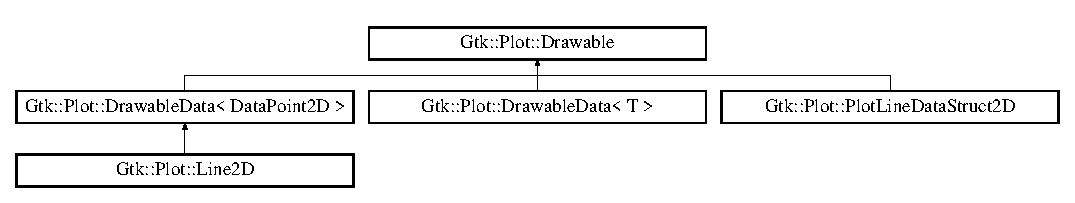
\includegraphics[height=2.28571cm]{classGtk_1_1Plot_1_1Drawable}
\end{center}
\end{figure}
\subsection*{Public Member Functions}
\begin{DoxyCompactItemize}
\item 
virtual void \hyperlink{classGtk_1_1Plot_1_1Drawable_ab1c723fcea852515f17d933e66b63ed2}{draw} (Cairo::RefPtr$<$ Cairo::Context $>$ context)=0
\item 
\hyperlink{classGtk_1_1Plot_1_1Drawable_a22c799e2e10a3f7b60df8568f0d78f20}{Drawable} ()
\item 
virtual \hyperlink{classGtk_1_1Plot_1_1Drawable_abae99caef51e103d2160ef9a61ca08f9}{$\sim$Drawable} ()
\end{DoxyCompactItemize}


\subsection{Constructor \& Destructor Documentation}
\hypertarget{classGtk_1_1Plot_1_1Drawable_a22c799e2e10a3f7b60df8568f0d78f20}{
\index{Gtk::Plot::Drawable@{Gtk::Plot::Drawable}!Drawable@{Drawable}}
\index{Drawable@{Drawable}!Gtk::Plot::Drawable@{Gtk::Plot::Drawable}}
\subsubsection[{Drawable}]{\setlength{\rightskip}{0pt plus 5cm}Gtk::Plot::Drawable::Drawable ()\hspace{0.3cm}{\ttfamily  \mbox{[}inline\mbox{]}}}}
\label{classGtk_1_1Plot_1_1Drawable_a22c799e2e10a3f7b60df8568f0d78f20}
\hypertarget{classGtk_1_1Plot_1_1Drawable_abae99caef51e103d2160ef9a61ca08f9}{
\index{Gtk::Plot::Drawable@{Gtk::Plot::Drawable}!$\sim$Drawable@{$\sim$Drawable}}
\index{$\sim$Drawable@{$\sim$Drawable}!Gtk::Plot::Drawable@{Gtk::Plot::Drawable}}
\subsubsection[{$\sim$Drawable}]{\setlength{\rightskip}{0pt plus 5cm}virtual Gtk::Plot::Drawable::$\sim$Drawable ()\hspace{0.3cm}{\ttfamily  \mbox{[}inline, virtual\mbox{]}}}}
\label{classGtk_1_1Plot_1_1Drawable_abae99caef51e103d2160ef9a61ca08f9}


\subsection{Member Function Documentation}
\hypertarget{classGtk_1_1Plot_1_1Drawable_ab1c723fcea852515f17d933e66b63ed2}{
\index{Gtk::Plot::Drawable@{Gtk::Plot::Drawable}!draw@{draw}}
\index{draw@{draw}!Gtk::Plot::Drawable@{Gtk::Plot::Drawable}}
\subsubsection[{draw}]{\setlength{\rightskip}{0pt plus 5cm}virtual void Gtk::Plot::Drawable::draw (Cairo::RefPtr$<$ Cairo::Context $>$ {\em context})\hspace{0.3cm}{\ttfamily  \mbox{[}pure virtual\mbox{]}}}}
\label{classGtk_1_1Plot_1_1Drawable_ab1c723fcea852515f17d933e66b63ed2}


Implemented in \hyperlink{classGtk_1_1Plot_1_1DrawableData_a275c0162df2dfdd060e859b63077614c}{Gtk::Plot::DrawableData$<$ T $>$}, \hyperlink{classGtk_1_1Plot_1_1Line2D_a4f5fc46b03bac4dc0a87fe7dd4945cf1}{Gtk::Plot::Line2D}, \hyperlink{structGtk_1_1Plot_1_1PlotLineDataStruct2D_ad3f4c1ed94cc37644032ac3be8995e1d}{Gtk::Plot::PlotLineDataStruct2D}, and \hyperlink{classGtk_1_1Plot_1_1DrawableData_a275c0162df2dfdd060e859b63077614c}{Gtk::Plot::DrawableData$<$ DataPoint2D $>$}.

The documentation for this class was generated from the following file:\begin{DoxyCompactItemize}
\item 
\hyperlink{types_8h}{types.h}\end{DoxyCompactItemize}

\hypertarget{classGtk_1_1Plot_1_1DrawableData}{
\section{Gtk::Plot::DrawableData$<$ T $>$ Class Template Reference}
\label{classGtk_1_1Plot_1_1DrawableData}\index{Gtk::Plot::DrawableData@{Gtk::Plot::DrawableData}}
}


{\ttfamily \#include $<$DrawableData.h$>$}Inheritance diagram for Gtk::Plot::DrawableData$<$ T $>$::\begin{figure}[H]
\begin{center}
\leavevmode
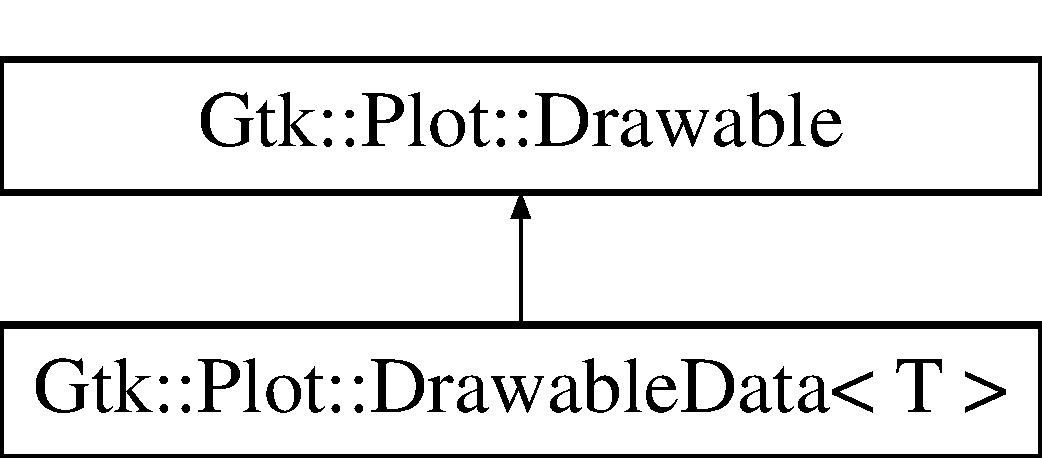
\includegraphics[height=2cm]{classGtk_1_1Plot_1_1DrawableData}
\end{center}
\end{figure}
\subsection*{Public Member Functions}
\begin{DoxyCompactItemize}
\item 
virtual int \hyperlink{classGtk_1_1Plot_1_1DrawableData_a7565034d7fa2fc8b9f230a3c792cecaa}{add\_\-data\_\-item} (T item)
\begin{DoxyCompactList}\small\item\em Pushes a data item onto the drawable stack. \item\end{DoxyCompactList}\item 
virtual void \hyperlink{classGtk_1_1Plot_1_1DrawableData_a275c0162df2dfdd060e859b63077614c}{draw} (Cairo::RefPtr$<$ Cairo::Context $>$ cr)
\begin{DoxyCompactList}\small\item\em Draw the data. \item\end{DoxyCompactList}\item 
\hyperlink{classGtk_1_1Plot_1_1DrawableData_a667213ec180f9292dfc6e57ddd63cd2b}{DrawableData} ()
\item 
virtual T \hyperlink{classGtk_1_1Plot_1_1DrawableData_aa36c69486f3b90c92a64ff9e26848858}{get\_\-data\_\-item} (int index)
\begin{DoxyCompactList}\small\item\em Retrieves a data item from the drawable stack. \item\end{DoxyCompactList}\item 
virtual T \hyperlink{classGtk_1_1Plot_1_1DrawableData_a94163585f0c15cdd71e293c19bcaecc4}{remove\_\-data\_\-item} (int index)
\begin{DoxyCompactList}\small\item\em Removes a data item from the drawable stack. \item\end{DoxyCompactList}\item 
virtual \hyperlink{classGtk_1_1Plot_1_1DrawableData_a56e3932c40f009ba2bea91c92a0f997a}{$\sim$DrawableData} ()
\end{DoxyCompactItemize}
\subsection*{Protected Attributes}
\begin{DoxyCompactItemize}
\item 
std::deque$<$ T $>$ \hyperlink{classGtk_1_1Plot_1_1DrawableData_ac8c6f3506d6286cfb432ed9a3f411c75}{m\_\-data\_\-set}
\item 
\hyperlink{namespaceGtk_1_1Plot_aa310e5a0b3e79b5d145978cdfdff19f7}{MarkerStyle} \hyperlink{classGtk_1_1Plot_1_1DrawableData_a4eb6eed74d1be1a72e093ce307b8f27f}{m\_\-marker\_\-style}
\end{DoxyCompactItemize}
\subsubsection*{template$<$typename T$>$ class Gtk::Plot::DrawableData$<$ T $>$}



\subsection{Constructor \& Destructor Documentation}
\hypertarget{classGtk_1_1Plot_1_1DrawableData_a667213ec180f9292dfc6e57ddd63cd2b}{
\index{Gtk::Plot::DrawableData@{Gtk::Plot::DrawableData}!DrawableData@{DrawableData}}
\index{DrawableData@{DrawableData}!Gtk::Plot::DrawableData@{Gtk::Plot::DrawableData}}
\subsubsection[{DrawableData}]{\setlength{\rightskip}{0pt plus 5cm}template$<$typename T$>$ {\bf Gtk::Plot::DrawableData}$<$ T $>$::{\bf DrawableData} ()\hspace{0.3cm}{\ttfamily  \mbox{[}inline\mbox{]}}}}
\label{classGtk_1_1Plot_1_1DrawableData_a667213ec180f9292dfc6e57ddd63cd2b}
\hypertarget{classGtk_1_1Plot_1_1DrawableData_a56e3932c40f009ba2bea91c92a0f997a}{
\index{Gtk::Plot::DrawableData@{Gtk::Plot::DrawableData}!$\sim$DrawableData@{$\sim$DrawableData}}
\index{$\sim$DrawableData@{$\sim$DrawableData}!Gtk::Plot::DrawableData@{Gtk::Plot::DrawableData}}
\subsubsection[{$\sim$DrawableData}]{\setlength{\rightskip}{0pt plus 5cm}template$<$typename T$>$ virtual {\bf Gtk::Plot::DrawableData}$<$ T $>$::$\sim${\bf DrawableData} ()\hspace{0.3cm}{\ttfamily  \mbox{[}inline, virtual\mbox{]}}}}
\label{classGtk_1_1Plot_1_1DrawableData_a56e3932c40f009ba2bea91c92a0f997a}


\subsection{Member Function Documentation}
\hypertarget{classGtk_1_1Plot_1_1DrawableData_a7565034d7fa2fc8b9f230a3c792cecaa}{
\index{Gtk::Plot::DrawableData@{Gtk::Plot::DrawableData}!add\_\-data\_\-item@{add\_\-data\_\-item}}
\index{add\_\-data\_\-item@{add\_\-data\_\-item}!Gtk::Plot::DrawableData@{Gtk::Plot::DrawableData}}
\subsubsection[{add\_\-data\_\-item}]{\setlength{\rightskip}{0pt plus 5cm}template$<$typename T$>$ int {\bf Gtk::Plot::DrawableData}$<$ T $>$::add\_\-data\_\-item (T {\em item})\hspace{0.3cm}{\ttfamily  \mbox{[}inline, virtual\mbox{]}}}}
\label{classGtk_1_1Plot_1_1DrawableData_a7565034d7fa2fc8b9f230a3c792cecaa}


Pushes a data item onto the drawable stack. 
\begin{DoxyParams}{Parameters}
\item[{\em item}]: item to push. \end{DoxyParams}
\hypertarget{classGtk_1_1Plot_1_1DrawableData_a275c0162df2dfdd060e859b63077614c}{
\index{Gtk::Plot::DrawableData@{Gtk::Plot::DrawableData}!draw@{draw}}
\index{draw@{draw}!Gtk::Plot::DrawableData@{Gtk::Plot::DrawableData}}
\subsubsection[{draw}]{\setlength{\rightskip}{0pt plus 5cm}template$<$typename T$>$ virtual void {\bf Gtk::Plot::DrawableData}$<$ T $>$::draw (Cairo::RefPtr$<$ Cairo::Context $>$ {\em cr})\hspace{0.3cm}{\ttfamily  \mbox{[}inline, virtual\mbox{]}}}}
\label{classGtk_1_1Plot_1_1DrawableData_a275c0162df2dfdd060e859b63077614c}


Draw the data. Note that that the context object passed to this method should already be prepared (sized, etc) as this method should only handle its own layout. 
\begin{DoxyParams}{Parameters}
\item[{\em cr}]: the cairo context to draw with. \end{DoxyParams}


Implements \hyperlink{classGtk_1_1Plot_1_1Drawable_ab1c723fcea852515f17d933e66b63ed2}{Gtk::Plot::Drawable}.

Reimplemented in \hyperlink{classGtk_1_1Plot_1_1Line2D_a4f5fc46b03bac4dc0a87fe7dd4945cf1}{Gtk::Plot::Line2D}.\hypertarget{classGtk_1_1Plot_1_1DrawableData_aa36c69486f3b90c92a64ff9e26848858}{
\index{Gtk::Plot::DrawableData@{Gtk::Plot::DrawableData}!get\_\-data\_\-item@{get\_\-data\_\-item}}
\index{get\_\-data\_\-item@{get\_\-data\_\-item}!Gtk::Plot::DrawableData@{Gtk::Plot::DrawableData}}
\subsubsection[{get\_\-data\_\-item}]{\setlength{\rightskip}{0pt plus 5cm}template$<$typename T $>$ T {\bf Gtk::Plot::DrawableData}$<$ T $>$::get\_\-data\_\-item (int {\em index})\hspace{0.3cm}{\ttfamily  \mbox{[}inline, virtual\mbox{]}}}}
\label{classGtk_1_1Plot_1_1DrawableData_aa36c69486f3b90c92a64ff9e26848858}


Retrieves a data item from the drawable stack. 
\begin{DoxyParams}{Parameters}
\item[{\em index}]: the item's index on the stack as returned by the add() method. \end{DoxyParams}
\begin{DoxyReturn}{Returns}
T : a data object of type T, as specified in constructor. $\ast$ 
\end{DoxyReturn}

\begin{DoxyExceptions}{Exceptions}
\item[{\em out\_\-of\_\-range}]if item was not found. \end{DoxyExceptions}
\hypertarget{classGtk_1_1Plot_1_1DrawableData_a94163585f0c15cdd71e293c19bcaecc4}{
\index{Gtk::Plot::DrawableData@{Gtk::Plot::DrawableData}!remove\_\-data\_\-item@{remove\_\-data\_\-item}}
\index{remove\_\-data\_\-item@{remove\_\-data\_\-item}!Gtk::Plot::DrawableData@{Gtk::Plot::DrawableData}}
\subsubsection[{remove\_\-data\_\-item}]{\setlength{\rightskip}{0pt plus 5cm}template$<$typename T $>$ T {\bf Gtk::Plot::DrawableData}$<$ T $>$::remove\_\-data\_\-item (int {\em index})\hspace{0.3cm}{\ttfamily  \mbox{[}inline, virtual\mbox{]}}}}
\label{classGtk_1_1Plot_1_1DrawableData_a94163585f0c15cdd71e293c19bcaecc4}


Removes a data item from the drawable stack. 
\begin{DoxyParams}{Parameters}
\item[{\em index}]: the item's index on the stack as returned by the add() method. \end{DoxyParams}
\begin{DoxyReturn}{Returns}
T : a data object of type T, as specified in constructor, if remove was successfull 
\end{DoxyReturn}

\begin{DoxyExceptions}{Exceptions}
\item[{\em out\_\-of\_\-range}]if item was not found. \end{DoxyExceptions}


\subsection{Member Data Documentation}
\hypertarget{classGtk_1_1Plot_1_1DrawableData_ac8c6f3506d6286cfb432ed9a3f411c75}{
\index{Gtk::Plot::DrawableData@{Gtk::Plot::DrawableData}!m\_\-data\_\-set@{m\_\-data\_\-set}}
\index{m\_\-data\_\-set@{m\_\-data\_\-set}!Gtk::Plot::DrawableData@{Gtk::Plot::DrawableData}}
\subsubsection[{m\_\-data\_\-set}]{\setlength{\rightskip}{0pt plus 5cm}template$<$typename T$>$ std::deque$<$T$>$ {\bf Gtk::Plot::DrawableData}$<$ T $>$::{\bf m\_\-data\_\-set}\hspace{0.3cm}{\ttfamily  \mbox{[}protected\mbox{]}}}}
\label{classGtk_1_1Plot_1_1DrawableData_ac8c6f3506d6286cfb432ed9a3f411c75}
\hypertarget{classGtk_1_1Plot_1_1DrawableData_a4eb6eed74d1be1a72e093ce307b8f27f}{
\index{Gtk::Plot::DrawableData@{Gtk::Plot::DrawableData}!m\_\-marker\_\-style@{m\_\-marker\_\-style}}
\index{m\_\-marker\_\-style@{m\_\-marker\_\-style}!Gtk::Plot::DrawableData@{Gtk::Plot::DrawableData}}
\subsubsection[{m\_\-marker\_\-style}]{\setlength{\rightskip}{0pt plus 5cm}template$<$typename T$>$ {\bf MarkerStyle} {\bf Gtk::Plot::DrawableData}$<$ T $>$::{\bf m\_\-marker\_\-style}\hspace{0.3cm}{\ttfamily  \mbox{[}protected\mbox{]}}}}
\label{classGtk_1_1Plot_1_1DrawableData_a4eb6eed74d1be1a72e093ce307b8f27f}


The documentation for this class was generated from the following file:\begin{DoxyCompactItemize}
\item 
\hyperlink{DrawableData_8h}{DrawableData.h}\end{DoxyCompactItemize}

\hypertarget{classGtk_1_1Plot_1_1Line2D}{
\section{Gtk::Plot::Line2D Class Reference}
\label{classGtk_1_1Plot_1_1Line2D}\index{Gtk::Plot::Line2D@{Gtk::Plot::Line2D}}
}


{\ttfamily \#include $<$Line2D.h$>$}Inheritance diagram for Gtk::Plot::Line2D::\begin{figure}[H]
\begin{center}
\leavevmode
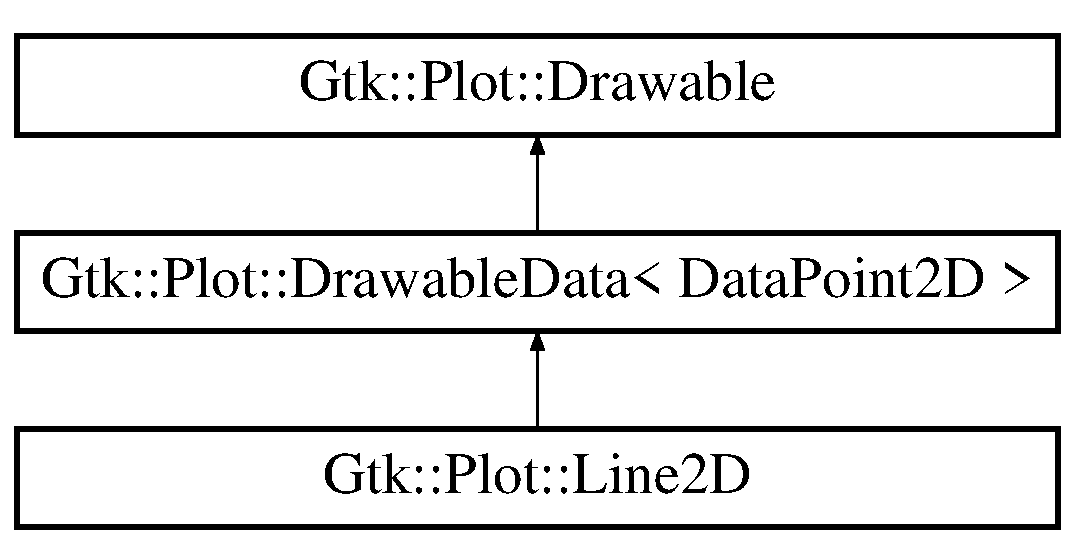
\includegraphics[height=3cm]{classGtk_1_1Plot_1_1Line2D}
\end{center}
\end{figure}
\subsection*{Public Member Functions}
\begin{DoxyCompactItemize}
\item 
void \hyperlink{classGtk_1_1Plot_1_1Line2D_a4f5fc46b03bac4dc0a87fe7dd4945cf1}{draw} (Cairo::RefPtr$<$ Cairo::Context $>$ cr)
\begin{DoxyCompactList}\small\item\em Draw the data. \item\end{DoxyCompactList}\item 
Gdk::Color $\ast$ \hyperlink{classGtk_1_1Plot_1_1Line2D_a29fb56ef0f66aa944d33f7327f5ab250}{get\_\-color} ()
\item 
std::valarray$<$ double $>$ $\ast$ \hyperlink{classGtk_1_1Plot_1_1Line2D_aca5b60a9b12895f64dba26d153c99785}{get\_\-dash} ()
\item 
double $\ast$ \hyperlink{classGtk_1_1Plot_1_1Line2D_a536017770621160e6e8c19c19b0485f2}{get\_\-width} ()
\item 
\hyperlink{classGtk_1_1Plot_1_1Line2D_af2f675904e4cdb37d958ad4d120798b4}{Line2D} ()
\item 
void \hyperlink{classGtk_1_1Plot_1_1Line2D_aeddda540e6d9c98d6495fdac8ceb7d3e}{set\_\-color} (Gdk::Color color)
\item 
void \hyperlink{classGtk_1_1Plot_1_1Line2D_ac569c4747dacde24d6d0e2fb4d9a2011}{set\_\-dash} (std::valarray$<$ double $>$ dash)
\item 
void \hyperlink{classGtk_1_1Plot_1_1Line2D_aa304dd085c71f0f85477f1680f0cafea}{set\_\-width} (double width)
\item 
virtual \hyperlink{classGtk_1_1Plot_1_1Line2D_abd9b0ace1e06932272a3dbd3f1009edf}{$\sim$Line2D} ()
\end{DoxyCompactItemize}
\subsection*{Protected Attributes}
\begin{DoxyCompactItemize}
\item 
Gdk::Color \hyperlink{classGtk_1_1Plot_1_1Line2D_ae322075b3cd8da490e47b3a0076d1b85}{m\_\-color}
\item 
std::valarray$<$ double $>$ \hyperlink{classGtk_1_1Plot_1_1Line2D_aa151e28045058d271b3f254cc078273e}{m\_\-dash}
\item 
double \hyperlink{classGtk_1_1Plot_1_1Line2D_a455d1610bfbfe269754464d2ba79cefb}{m\_\-width}
\end{DoxyCompactItemize}


\subsection{Constructor \& Destructor Documentation}
\hypertarget{classGtk_1_1Plot_1_1Line2D_af2f675904e4cdb37d958ad4d120798b4}{
\index{Gtk::Plot::Line2D@{Gtk::Plot::Line2D}!Line2D@{Line2D}}
\index{Line2D@{Line2D}!Gtk::Plot::Line2D@{Gtk::Plot::Line2D}}
\subsubsection[{Line2D}]{\setlength{\rightskip}{0pt plus 5cm}Gtk::Plot::Line2D::Line2D ()}}
\label{classGtk_1_1Plot_1_1Line2D_af2f675904e4cdb37d958ad4d120798b4}
\hypertarget{classGtk_1_1Plot_1_1Line2D_abd9b0ace1e06932272a3dbd3f1009edf}{
\index{Gtk::Plot::Line2D@{Gtk::Plot::Line2D}!$\sim$Line2D@{$\sim$Line2D}}
\index{$\sim$Line2D@{$\sim$Line2D}!Gtk::Plot::Line2D@{Gtk::Plot::Line2D}}
\subsubsection[{$\sim$Line2D}]{\setlength{\rightskip}{0pt plus 5cm}Gtk::Plot::Line2D::$\sim$Line2D ()\hspace{0.3cm}{\ttfamily  \mbox{[}virtual\mbox{]}}}}
\label{classGtk_1_1Plot_1_1Line2D_abd9b0ace1e06932272a3dbd3f1009edf}


\subsection{Member Function Documentation}
\hypertarget{classGtk_1_1Plot_1_1Line2D_a4f5fc46b03bac4dc0a87fe7dd4945cf1}{
\index{Gtk::Plot::Line2D@{Gtk::Plot::Line2D}!draw@{draw}}
\index{draw@{draw}!Gtk::Plot::Line2D@{Gtk::Plot::Line2D}}
\subsubsection[{draw}]{\setlength{\rightskip}{0pt plus 5cm}void Gtk::Plot::Line2D::draw (Cairo::RefPtr$<$ Cairo::Context $>$ {\em cr})\hspace{0.3cm}{\ttfamily  \mbox{[}virtual\mbox{]}}}}
\label{classGtk_1_1Plot_1_1Line2D_a4f5fc46b03bac4dc0a87fe7dd4945cf1}


Draw the data. Note that that the context object passed to this method should already be prepared (sized, etc) as this method should only handle its own layout. 
\begin{DoxyParams}{Parameters}
\item[{\em cr}]: the cairo context to draw with. \end{DoxyParams}


Reimplemented from \hyperlink{classGtk_1_1Plot_1_1DrawableData_a275c0162df2dfdd060e859b63077614c}{Gtk::Plot::DrawableData$<$ DataPoint2D $>$}.\hypertarget{classGtk_1_1Plot_1_1Line2D_a29fb56ef0f66aa944d33f7327f5ab250}{
\index{Gtk::Plot::Line2D@{Gtk::Plot::Line2D}!get\_\-color@{get\_\-color}}
\index{get\_\-color@{get\_\-color}!Gtk::Plot::Line2D@{Gtk::Plot::Line2D}}
\subsubsection[{get\_\-color}]{\setlength{\rightskip}{0pt plus 5cm}Gdk::Color $\ast$ Gtk::Plot::Line2D::get\_\-color ()}}
\label{classGtk_1_1Plot_1_1Line2D_a29fb56ef0f66aa944d33f7327f5ab250}
\hypertarget{classGtk_1_1Plot_1_1Line2D_aca5b60a9b12895f64dba26d153c99785}{
\index{Gtk::Plot::Line2D@{Gtk::Plot::Line2D}!get\_\-dash@{get\_\-dash}}
\index{get\_\-dash@{get\_\-dash}!Gtk::Plot::Line2D@{Gtk::Plot::Line2D}}
\subsubsection[{get\_\-dash}]{\setlength{\rightskip}{0pt plus 5cm}std::valarray$<$ double $>$ $\ast$ Gtk::Plot::Line2D::get\_\-dash ()}}
\label{classGtk_1_1Plot_1_1Line2D_aca5b60a9b12895f64dba26d153c99785}
\hypertarget{classGtk_1_1Plot_1_1Line2D_a536017770621160e6e8c19c19b0485f2}{
\index{Gtk::Plot::Line2D@{Gtk::Plot::Line2D}!get\_\-width@{get\_\-width}}
\index{get\_\-width@{get\_\-width}!Gtk::Plot::Line2D@{Gtk::Plot::Line2D}}
\subsubsection[{get\_\-width}]{\setlength{\rightskip}{0pt plus 5cm}double $\ast$ Gtk::Plot::Line2D::get\_\-width ()}}
\label{classGtk_1_1Plot_1_1Line2D_a536017770621160e6e8c19c19b0485f2}
\hypertarget{classGtk_1_1Plot_1_1Line2D_aeddda540e6d9c98d6495fdac8ceb7d3e}{
\index{Gtk::Plot::Line2D@{Gtk::Plot::Line2D}!set\_\-color@{set\_\-color}}
\index{set\_\-color@{set\_\-color}!Gtk::Plot::Line2D@{Gtk::Plot::Line2D}}
\subsubsection[{set\_\-color}]{\setlength{\rightskip}{0pt plus 5cm}void Gtk::Plot::Line2D::set\_\-color (Gdk::Color {\em color})}}
\label{classGtk_1_1Plot_1_1Line2D_aeddda540e6d9c98d6495fdac8ceb7d3e}
\hypertarget{classGtk_1_1Plot_1_1Line2D_ac569c4747dacde24d6d0e2fb4d9a2011}{
\index{Gtk::Plot::Line2D@{Gtk::Plot::Line2D}!set\_\-dash@{set\_\-dash}}
\index{set\_\-dash@{set\_\-dash}!Gtk::Plot::Line2D@{Gtk::Plot::Line2D}}
\subsubsection[{set\_\-dash}]{\setlength{\rightskip}{0pt plus 5cm}void Gtk::Plot::Line2D::set\_\-dash (std::valarray$<$ double $>$ {\em dash})}}
\label{classGtk_1_1Plot_1_1Line2D_ac569c4747dacde24d6d0e2fb4d9a2011}
\hypertarget{classGtk_1_1Plot_1_1Line2D_aa304dd085c71f0f85477f1680f0cafea}{
\index{Gtk::Plot::Line2D@{Gtk::Plot::Line2D}!set\_\-width@{set\_\-width}}
\index{set\_\-width@{set\_\-width}!Gtk::Plot::Line2D@{Gtk::Plot::Line2D}}
\subsubsection[{set\_\-width}]{\setlength{\rightskip}{0pt plus 5cm}void Gtk::Plot::Line2D::set\_\-width (double {\em width})}}
\label{classGtk_1_1Plot_1_1Line2D_aa304dd085c71f0f85477f1680f0cafea}


\subsection{Member Data Documentation}
\hypertarget{classGtk_1_1Plot_1_1Line2D_ae322075b3cd8da490e47b3a0076d1b85}{
\index{Gtk::Plot::Line2D@{Gtk::Plot::Line2D}!m\_\-color@{m\_\-color}}
\index{m\_\-color@{m\_\-color}!Gtk::Plot::Line2D@{Gtk::Plot::Line2D}}
\subsubsection[{m\_\-color}]{\setlength{\rightskip}{0pt plus 5cm}Gdk::Color {\bf Gtk::Plot::Line2D::m\_\-color}\hspace{0.3cm}{\ttfamily  \mbox{[}protected\mbox{]}}}}
\label{classGtk_1_1Plot_1_1Line2D_ae322075b3cd8da490e47b3a0076d1b85}
\hypertarget{classGtk_1_1Plot_1_1Line2D_aa151e28045058d271b3f254cc078273e}{
\index{Gtk::Plot::Line2D@{Gtk::Plot::Line2D}!m\_\-dash@{m\_\-dash}}
\index{m\_\-dash@{m\_\-dash}!Gtk::Plot::Line2D@{Gtk::Plot::Line2D}}
\subsubsection[{m\_\-dash}]{\setlength{\rightskip}{0pt plus 5cm}std::valarray$<$double$>$ {\bf Gtk::Plot::Line2D::m\_\-dash}\hspace{0.3cm}{\ttfamily  \mbox{[}protected\mbox{]}}}}
\label{classGtk_1_1Plot_1_1Line2D_aa151e28045058d271b3f254cc078273e}
\hypertarget{classGtk_1_1Plot_1_1Line2D_a455d1610bfbfe269754464d2ba79cefb}{
\index{Gtk::Plot::Line2D@{Gtk::Plot::Line2D}!m\_\-width@{m\_\-width}}
\index{m\_\-width@{m\_\-width}!Gtk::Plot::Line2D@{Gtk::Plot::Line2D}}
\subsubsection[{m\_\-width}]{\setlength{\rightskip}{0pt plus 5cm}double {\bf Gtk::Plot::Line2D::m\_\-width}\hspace{0.3cm}{\ttfamily  \mbox{[}protected\mbox{]}}}}
\label{classGtk_1_1Plot_1_1Line2D_a455d1610bfbfe269754464d2ba79cefb}


The documentation for this class was generated from the following files:\begin{DoxyCompactItemize}
\item 
\hyperlink{Line2D_8h}{Line2D.h}\item 
\hyperlink{Line2D_8cpp}{Line2D.cpp}\end{DoxyCompactItemize}

\hypertarget{structGtk_1_1Plot_1_1PlotLineDataStruct2D}{
\section{Gtk::Plot::PlotLineDataStruct2D Struct Reference}
\label{structGtk_1_1Plot_1_1PlotLineDataStruct2D}\index{Gtk::Plot::PlotLineDataStruct2D@{Gtk::Plot::PlotLineDataStruct2D}}
}


{\ttfamily \#include $<$types.h$>$}Inheritance diagram for Gtk::Plot::PlotLineDataStruct2D::\begin{figure}[H]
\begin{center}
\leavevmode
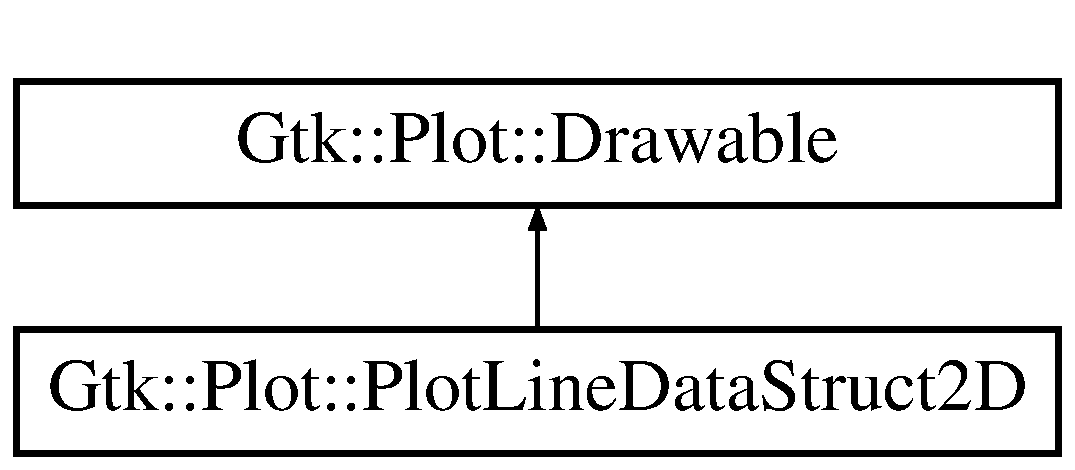
\includegraphics[height=2cm]{structGtk_1_1Plot_1_1PlotLineDataStruct2D}
\end{center}
\end{figure}
\subsection*{Public Member Functions}
\begin{DoxyCompactItemize}
\item 
void \hyperlink{structGtk_1_1Plot_1_1PlotLineDataStruct2D_ad3f4c1ed94cc37644032ac3be8995e1d}{draw} (Cairo::RefPtr$<$ Cairo::Context $>$ context)
\item 
\hyperlink{structGtk_1_1Plot_1_1PlotLineDataStruct2D_a3f2f9b4ec89a940baea3c1fd3e0da75e}{PlotLineDataStruct2D} (double \hyperlink{structGtk_1_1Plot_1_1PlotLineDataStruct2D_abc9c02f23c4bd8cdb29bc3c497ca121b}{x}, double \hyperlink{structGtk_1_1Plot_1_1PlotLineDataStruct2D_a9a13b8cff1bbb4428b1affe716379e0d}{y})
\end{DoxyCompactItemize}
\subsection*{Public Attributes}
\begin{DoxyCompactItemize}
\item 
double \hyperlink{structGtk_1_1Plot_1_1PlotLineDataStruct2D_abc9c02f23c4bd8cdb29bc3c497ca121b}{x}
\item 
double \hyperlink{structGtk_1_1Plot_1_1PlotLineDataStruct2D_a9a13b8cff1bbb4428b1affe716379e0d}{y}
\end{DoxyCompactItemize}


\subsection{Constructor \& Destructor Documentation}
\hypertarget{structGtk_1_1Plot_1_1PlotLineDataStruct2D_a3f2f9b4ec89a940baea3c1fd3e0da75e}{
\index{Gtk::Plot::PlotLineDataStruct2D@{Gtk::Plot::PlotLineDataStruct2D}!PlotLineDataStruct2D@{PlotLineDataStruct2D}}
\index{PlotLineDataStruct2D@{PlotLineDataStruct2D}!Gtk::Plot::PlotLineDataStruct2D@{Gtk::Plot::PlotLineDataStruct2D}}
\subsubsection[{PlotLineDataStruct2D}]{\setlength{\rightskip}{0pt plus 5cm}Gtk::Plot::PlotLineDataStruct2D::PlotLineDataStruct2D (double {\em x}, \/  double {\em y})\hspace{0.3cm}{\ttfamily  \mbox{[}inline\mbox{]}}}}
\label{structGtk_1_1Plot_1_1PlotLineDataStruct2D_a3f2f9b4ec89a940baea3c1fd3e0da75e}


\subsection{Member Function Documentation}
\hypertarget{structGtk_1_1Plot_1_1PlotLineDataStruct2D_ad3f4c1ed94cc37644032ac3be8995e1d}{
\index{Gtk::Plot::PlotLineDataStruct2D@{Gtk::Plot::PlotLineDataStruct2D}!draw@{draw}}
\index{draw@{draw}!Gtk::Plot::PlotLineDataStruct2D@{Gtk::Plot::PlotLineDataStruct2D}}
\subsubsection[{draw}]{\setlength{\rightskip}{0pt plus 5cm}void Gtk::Plot::PlotLineDataStruct2D::draw (Cairo::RefPtr$<$ Cairo::Context $>$ {\em context})\hspace{0.3cm}{\ttfamily  \mbox{[}inline, virtual\mbox{]}}}}
\label{structGtk_1_1Plot_1_1PlotLineDataStruct2D_ad3f4c1ed94cc37644032ac3be8995e1d}


Implements \hyperlink{classGtk_1_1Plot_1_1Drawable_ab1c723fcea852515f17d933e66b63ed2}{Gtk::Plot::Drawable}.

\subsection{Member Data Documentation}
\hypertarget{structGtk_1_1Plot_1_1PlotLineDataStruct2D_abc9c02f23c4bd8cdb29bc3c497ca121b}{
\index{Gtk::Plot::PlotLineDataStruct2D@{Gtk::Plot::PlotLineDataStruct2D}!x@{x}}
\index{x@{x}!Gtk::Plot::PlotLineDataStruct2D@{Gtk::Plot::PlotLineDataStruct2D}}
\subsubsection[{x}]{\setlength{\rightskip}{0pt plus 5cm}double {\bf Gtk::Plot::PlotLineDataStruct2D::x}}}
\label{structGtk_1_1Plot_1_1PlotLineDataStruct2D_abc9c02f23c4bd8cdb29bc3c497ca121b}
\hypertarget{structGtk_1_1Plot_1_1PlotLineDataStruct2D_a9a13b8cff1bbb4428b1affe716379e0d}{
\index{Gtk::Plot::PlotLineDataStruct2D@{Gtk::Plot::PlotLineDataStruct2D}!y@{y}}
\index{y@{y}!Gtk::Plot::PlotLineDataStruct2D@{Gtk::Plot::PlotLineDataStruct2D}}
\subsubsection[{y}]{\setlength{\rightskip}{0pt plus 5cm}double {\bf Gtk::Plot::PlotLineDataStruct2D::y}}}
\label{structGtk_1_1Plot_1_1PlotLineDataStruct2D_a9a13b8cff1bbb4428b1affe716379e0d}


The documentation for this struct was generated from the following file:\begin{DoxyCompactItemize}
\item 
\hyperlink{types_8h}{types.h}\end{DoxyCompactItemize}

\chapter{File Documentation}
\hypertarget{DrawableData_8cpp}{
\section{DrawableData.cpp File Reference}
\label{DrawableData_8cpp}\index{DrawableData.cpp@{DrawableData.cpp}}
}
{\ttfamily \#include $<$stdexcept$>$}\par
{\ttfamily \#include \char`\"{}DrawableData.h\char`\"{}}\par
\subsection*{Namespaces}
\begin{DoxyCompactItemize}
\item 
namespace \hyperlink{namespaceGtk}{Gtk}
\item 
namespace \hyperlink{namespaceGtk_1_1Plot}{Gtk::Plot}
\end{DoxyCompactItemize}

\hypertarget{DrawableData_8h}{
\section{DrawableData.h File Reference}
\label{DrawableData_8h}\index{DrawableData.h@{DrawableData.h}}
}
{\ttfamily \#include $<$deque$>$}\par
{\ttfamily \#include $<$cairomm-\/1.0/cairomm/context.h$>$}\par
{\ttfamily \#include $<$cairomm-\/1.0/cairomm/refptr.h$>$}\par
{\ttfamily \#include \char`\"{}types.h\char`\"{}}\par
\subsection*{Classes}
\begin{DoxyCompactItemize}
\item 
class \hyperlink{classGtk_1_1Plot_1_1DrawableData}{Gtk::Plot::DrawableData$<$ T $>$}
\end{DoxyCompactItemize}
\subsection*{Namespaces}
\begin{DoxyCompactItemize}
\item 
namespace \hyperlink{namespaceGtk}{Gtk}
\item 
namespace \hyperlink{namespaceGtk_1_1Plot}{Gtk::Plot}
\end{DoxyCompactItemize}

\hypertarget{Line2D_8cpp}{
\section{Line2D.cpp File Reference}
\label{Line2D_8cpp}\index{Line2D.cpp@{Line2D.cpp}}
}
{\ttfamily \#include $<$iostream$>$}\par
{\ttfamily \#include $<$gdkmm-\/2.4/gdkmm.h$>$}\par
{\ttfamily \#include $<$gdkmm-\/2.4/gdkmm/general.h$>$}\par
{\ttfamily \#include \char`\"{}Line2D.h\char`\"{}}\par
\subsection*{Namespaces}
\begin{DoxyCompactItemize}
\item 
namespace \hyperlink{namespaceGtk}{Gtk}
\item 
namespace \hyperlink{namespaceGtk_1_1Plot}{Gtk::Plot}
\end{DoxyCompactItemize}

\hypertarget{Line2D_8h}{
\section{Line2D.h File Reference}
\label{Line2D_8h}\index{Line2D.h@{Line2D.h}}
}
{\ttfamily \#include \char`\"{}types.h\char`\"{}}\par
{\ttfamily \#include \char`\"{}DrawableData.h\char`\"{}}\par
\subsection*{Classes}
\begin{DoxyCompactItemize}
\item 
class \hyperlink{classGtk_1_1Plot_1_1Line2D}{Gtk::Plot::Line2D}
\end{DoxyCompactItemize}
\subsection*{Namespaces}
\begin{DoxyCompactItemize}
\item 
namespace \hyperlink{namespaceGtk}{Gtk}
\item 
namespace \hyperlink{namespaceGtk_1_1Plot}{Gtk::Plot}
\end{DoxyCompactItemize}

\hypertarget{PlotArea_8cpp}{
\section{PlotArea.cpp File Reference}
\label{PlotArea_8cpp}\index{PlotArea.cpp@{PlotArea.cpp}}
}
{\ttfamily \#include $<$vector$>$}\par
{\ttfamily \#include $<$cairomm-\/1.0/cairomm/context.h$>$}\par
{\ttfamily \#include $<$cairomm-\/1.0/cairomm/refptr.h$>$}\par
{\ttfamily \#include $<$gdkmm-\/2.4/gdkmm.h$>$}\par
{\ttfamily \#include $<$gdkmm-\/2.4/gdkmm/general.h$>$}\par
{\ttfamily \#include $<$pangomm-\/1.4/pangomm/fontdescription.h$>$}\par
{\ttfamily \#include $<$pangomm-\/1.4/pangomm/layout.h$>$}\par
{\ttfamily \#include $<$pangomm-\/1.4/pangomm/types.h$>$}\par
{\ttfamily \#include \char`\"{}PlotArea.h\char`\"{}}\par
{\ttfamily \#include \char`\"{}Line2D.h\char`\"{}}\par
\subsection*{Namespaces}
\begin{DoxyCompactItemize}
\item 
namespace \hyperlink{namespaceGtk}{Gtk}
\item 
namespace \hyperlink{namespaceGtk_1_1Plot}{Gtk::Plot}
\end{DoxyCompactItemize}

\hypertarget{PlotArea_8h}{
\section{PlotArea.h File Reference}
\label{PlotArea_8h}\index{PlotArea.h@{PlotArea.h}}
}
{\ttfamily \#include $<$deque$>$}\par
{\ttfamily \#include $<$string$>$}\par
{\ttfamily \#include $<$cairomm-\/1.0/cairomm/matrix.h$>$}\par
{\ttfamily \#include $<$gtk-\/2.0/gdk/gdkevents.h$>$}\par
{\ttfamily \#include $<$gtk-\/2.0/gtk/gtkobject.h$>$}\par
{\ttfamily \#include $<$gdkmm-\/2.4/gdkmm/rectangle.h$>$}\par
{\ttfamily \#include $<$gtkmm-\/2.4/gtkmm/drawingarea.h$>$}\par
{\ttfamily \#include $<$gtkmm-\/2.4/gtkmm/widget.h$>$}\par
{\ttfamily \#include $<$gtkmm-\/2.4/gtkmm/label.h$>$}\par
{\ttfamily \#include \char`\"{}types.h\char`\"{}}\par
{\ttfamily \#include \char`\"{}DrawableData.h\char`\"{}}\par
{\ttfamily \#include \char`\"{}Line2D.h\char`\"{}}\par
\subsection*{Classes}
\begin{DoxyCompactItemize}
\item 
class \hyperlink{classGtk_1_1Plot_1_1Area}{Gtk::Plot::Area}
\end{DoxyCompactItemize}
\subsection*{Namespaces}
\begin{DoxyCompactItemize}
\item 
namespace \hyperlink{namespaceGtk}{Gtk}
\item 
namespace \hyperlink{namespaceGtk_1_1Plot}{Gtk::Plot}
\end{DoxyCompactItemize}

\hypertarget{PlotContainer_8cpp}{
\section{PlotContainer.cpp File Reference}
\label{PlotContainer_8cpp}\index{PlotContainer.cpp@{PlotContainer.cpp}}
}
{\ttfamily \#include \char`\"{}PlotContainer.h\char`\"{}}\par
\subsection*{Namespaces}
\begin{DoxyCompactItemize}
\item 
namespace \hyperlink{namespaceGtk}{Gtk}
\item 
namespace \hyperlink{namespaceGtk_1_1Plot}{Gtk::Plot}
\end{DoxyCompactItemize}

\hypertarget{PlotContainer_8h}{
\section{PlotContainer.h File Reference}
\label{PlotContainer_8h}\index{PlotContainer.h@{PlotContainer.h}}
}
{\ttfamily \#include $<$gtk-\/2.0/gtk/gtkobject.h$>$}\par
{\ttfamily \#include $<$gtkmm-\/2.4/gtkmm/container.h$>$}\par
{\ttfamily \#include $<$gtkmm-\/2.4/gtkmm/widget.h$>$}\par
{\ttfamily \#include \char`\"{}PlotArea.h\char`\"{}}\par
\subsection*{Classes}
\begin{DoxyCompactItemize}
\item 
class \hyperlink{classGtk_1_1Plot_1_1Container}{Gtk::Plot::Container}
\end{DoxyCompactItemize}
\subsection*{Namespaces}
\begin{DoxyCompactItemize}
\item 
namespace \hyperlink{namespaceGtk}{Gtk}
\item 
namespace \hyperlink{namespaceGtk_1_1Plot}{Gtk::Plot}
\end{DoxyCompactItemize}

\hypertarget{types_8h}{
\section{types.h File Reference}
\label{types_8h}\index{types.h@{types.h}}
}
{\ttfamily \#include $<$gdkmm-\/2.4/gdkmm/color.h$>$}\par
{\ttfamily \#include $<$gtkmm-\/2.4/gtkmm/enums.h$>$}\par
{\ttfamily \#include $<$cairomm-\/1.0/cairomm/context.h$>$}\par
{\ttfamily \#include $<$cairomm-\/1.0/cairomm/refptr.h$>$}\par
\subsection*{Classes}
\begin{DoxyCompactItemize}
\item 
struct \hyperlink{structGtk_1_1Plot_1_1Border}{Gtk::Plot::Border}
\item 
class \hyperlink{classGtk_1_1Plot_1_1Drawable}{Gtk::Plot::Drawable}
\item 
struct \hyperlink{structGtk_1_1Plot_1_1PlotLineDataStruct2D}{Gtk::Plot::PlotLineDataStruct2D}
\end{DoxyCompactItemize}
\subsection*{Namespaces}
\begin{DoxyCompactItemize}
\item 
namespace \hyperlink{namespaceGtk}{Gtk}
\item 
namespace \hyperlink{namespaceGtk_1_1Plot}{Gtk::Plot}
\end{DoxyCompactItemize}
\subsection*{Typedefs}
\begin{DoxyCompactItemize}
\item 
typedef \hyperlink{structGtk_1_1Plot_1_1PlotLineDataStruct2D}{Gtk::Plot::PlotLineDataStruct2D} \hyperlink{namespaceGtk_1_1Plot_abea92d3a790b1bcf6a64f98511231815}{Gtk::Plot::DataPoint2D}
\item 
typedef Border \hyperlink{namespaceGtk_1_1Plot_a9b9ee0ab9bbec47945b0bf70f30ea308}{Gtk::Plot::Line}
\end{DoxyCompactItemize}
\subsection*{Enumerations}
\begin{DoxyCompactItemize}
\item 
enum \hyperlink{namespaceGtk_1_1Plot_aa7cadb8fb1ada346afe4e3acce74600d}{Gtk::Plot::DefaultVector} \{ \hyperlink{namespaceGtk_1_1Plot_aa7cadb8fb1ada346afe4e3acce74600da9d3e2fcd8a264bb72f0a74985c3590f0}{Gtk::Plot::VECTOR\_\-TOP\_\-LEFT} =  Gtk::CORNER\_\-TOP\_\-LEFT, 
\hyperlink{namespaceGtk_1_1Plot_aa7cadb8fb1ada346afe4e3acce74600da13009b468d527c2d59db116671bf86c8}{Gtk::Plot::VECTOR\_\-BOTTOM\_\-LEFT} =  Gtk::CORNER\_\-BOTTOM\_\-LEFT, 
\hyperlink{namespaceGtk_1_1Plot_aa7cadb8fb1ada346afe4e3acce74600da065d3f313fe6f3dd4bf0d1c01640cad4}{Gtk::Plot::VECTOR\_\-BOTTOM\_\-RIGHT} =  Gtk::CORNER\_\-BOTTOM\_\-RIGHT, 
\hyperlink{namespaceGtk_1_1Plot_aa7cadb8fb1ada346afe4e3acce74600da7472334ab3130df5927bb5b68f131da3}{Gtk::Plot::VECTOR\_\-TOP\_\-RIGHT} =  Gtk::CORNER\_\-TOP\_\-RIGHT
 \}
\item 
enum \hyperlink{namespaceGtk_1_1Plot_a125746674247df0f29cb6d6aa8089cb6}{Gtk::Plot::LabelPosition} \{ \hyperlink{namespaceGtk_1_1Plot_a125746674247df0f29cb6d6aa8089cb6af6133ad5c0f9a706cf047dc48739c991}{Gtk::Plot::POSITION\_\-INNER} =  0, 
\hyperlink{namespaceGtk_1_1Plot_a125746674247df0f29cb6d6aa8089cb6a848fbccbbfc3d4766f150d90be1e1026}{Gtk::Plot::POSITION\_\-OUTER} =  1, 
\hyperlink{namespaceGtk_1_1Plot_a125746674247df0f29cb6d6aa8089cb6aa5184b4fdfaa911c4a8cf87146df076c}{Gtk::Plot::POSITION\_\-DEFAULT} =  1
 \}
\item 
enum \hyperlink{namespaceGtk_1_1Plot_aa310e5a0b3e79b5d145978cdfdff19f7}{Gtk::Plot::MarkerStyle} \{ \par
\hyperlink{namespaceGtk_1_1Plot_aa310e5a0b3e79b5d145978cdfdff19f7a618d8963f2cb32284cd9584825a0f016}{Gtk::Plot::MARKER\_\-NONE} =  0, 
\hyperlink{namespaceGtk_1_1Plot_aa310e5a0b3e79b5d145978cdfdff19f7a9957a1ee0bda0fc1c63f77ced5fe218d}{Gtk::Plot::MARKER\_\-DOT} =  1, 
\hyperlink{namespaceGtk_1_1Plot_aa310e5a0b3e79b5d145978cdfdff19f7a9679ebd9735aae8ae32369be46fbe529}{Gtk::Plot::MARKER\_\-TRIANGLE} =  2, 
\hyperlink{namespaceGtk_1_1Plot_aa310e5a0b3e79b5d145978cdfdff19f7a2ec925d03c26998ddb10b5388c454e88}{Gtk::Plot::MARKER\_\-SQUARE} =  3, 
\par
\hyperlink{namespaceGtk_1_1Plot_aa310e5a0b3e79b5d145978cdfdff19f7a14412a86fb1eea3b0fa66b4f3496b1f9}{Gtk::Plot::MARKER\_\-CIRCLE} =  4, 
\hyperlink{namespaceGtk_1_1Plot_aa310e5a0b3e79b5d145978cdfdff19f7af0fa8bae0062c6ab61310baac3bc2af1}{Gtk::Plot::MARKER\_\-CROSSHAIR} =  5, 
\hyperlink{namespaceGtk_1_1Plot_aa310e5a0b3e79b5d145978cdfdff19f7a981911cfdb0e03eed0a82b502975c9f0}{Gtk::Plot::MARKER\_\-DEFAULT} =  MARKER\_\-NONE
 \}
\item 
enum \hyperlink{namespaceGtk_1_1Plot_a0ce4e6f495df606dd5b947ea1512490f}{Gtk::Plot::Origin} \{ \par
\hyperlink{namespaceGtk_1_1Plot_a0ce4e6f495df606dd5b947ea1512490fa98fa5422cd004789dd6ffa177dbbf9c1}{Gtk::Plot::TOP\_\-LEFT} =  Gtk::CORNER\_\-TOP\_\-LEFT, 
\hyperlink{namespaceGtk_1_1Plot_a0ce4e6f495df606dd5b947ea1512490fae8c1087d3c4fb149d4a01649b3922526}{Gtk::Plot::BOTTOM\_\-LEFT} =  Gtk::CORNER\_\-BOTTOM\_\-LEFT, 
\hyperlink{namespaceGtk_1_1Plot_a0ce4e6f495df606dd5b947ea1512490fa0c3adfc8278441f683b401245ec66130}{Gtk::Plot::BOTTOM\_\-RIGHT} =  Gtk::CORNER\_\-BOTTOM\_\-RIGHT, 
\hyperlink{namespaceGtk_1_1Plot_a0ce4e6f495df606dd5b947ea1512490fa8615d5a4ef038ffb006b7a6dc3d07101}{Gtk::Plot::TOP\_\-RIGHT} =  Gtk::CORNER\_\-TOP\_\-RIGHT, 
\par
\hyperlink{namespaceGtk_1_1Plot_a0ce4e6f495df606dd5b947ea1512490fa10b97cf832233cb157c484900e6375af}{Gtk::Plot::CENTER} =  10, 
\hyperlink{namespaceGtk_1_1Plot_a0ce4e6f495df606dd5b947ea1512490faec9bc95faf6c238679ed5c2c6338185f}{Gtk::Plot::CAIRO\_\-DEFAULT} =  TOP\_\-LEFT
 \}
\end{DoxyCompactItemize}

\printindex
\end{document}
